%
%% Default to the notebook output style
%
%    
%
%
%% Inherit from the specified cell style.    
%\documentclass[11pt]{article}
%
%    
%    
%    \usepackage[T1]{fontenc}
%    % Nicer default font (+ math font) than Computer Modern for most use cases
%    \usepackage{mathpazo}
%
%    % Basic figure setup, for now with no caption control since it's done
%    % automatically by Pandoc (which extracts ![](path) syntax from Markdown).
%    \usepackage{graphicx}
%    % We will generate all images so they have a width \maxwidth. This means
%    % that they will get their normal width if they fit onto the page, but
%    % are scaled down if they would overflow the margins.
%    \makeatletter
%    \def\maxwidth{\ifdim\Gin@nat@width>\linewidth\linewidth
%    \else\Gin@nat@width\fi}
%    \makeatother
%    \let\Oldincludegraphics\includegraphics
%    % Set max figure width to be 80% of text width, for now hardcoded.
%    \renewcommand{\includegraphics}[1]{\Oldincludegraphics[width=.8\maxwidth]{#1}}
%    % Ensure that by default, figures have no caption (until we provide a
%    % proper Figure object with a Caption API and a way to capture that
%    % in the conversion process - todo).
%    \usepackage{caption}
%    \DeclareCaptionLabelFormat{nolabel}{}
%    \captionsetup{labelformat=nolabel}
%
%    \usepackage{adjustbox} % Used to constrain images to a maximum size 
%    \usepackage{xcolor} % Allow colors to be defined
%    \usepackage{enumerate} % Needed for markdown enumerations to work
%    \usepackage{geometry} % Used to adjust the document margins
%    \usepackage{amsmath} % Equations
%    \usepackage{amssymb} % Equations
%    \usepackage{textcomp} % defines textquotesingle
%    % Hack from http://tex.stackexchange.com/a/47451/13684:
%    \AtBeginDocument{%
%        \def\PYZsq{\textquotesingle}% Upright quotes in Pygmentized code
%    }
%    \usepackage{upquote} % Upright quotes for verbatim code
%    \usepackage{eurosym} % defines \euro
%    \usepackage[mathletters]{ucs} % Extended unicode (utf-8) support
%    \usepackage[utf8x]{inputenc} % Allow utf-8 characters in the tex document
%    \usepackage{fancyvrb} % verbatim replacement that allows latex
%    \usepackage{grffile} % extends the file name processing of package graphics 
%                         % to support a larger range 
%    % The hyperref package gives us a pdf with properly built
%    % internal navigation ('pdf bookmarks' for the table of contents,
%    % internal cross-reference links, web links for URLs, etc.)
%    \usepackage{hyperref}
%    \usepackage{longtable} % longtable support required by pandoc >1.10
%    \usepackage{booktabs}  % table support for pandoc > 1.12.2
%    \usepackage[inline]{enumitem} % IRkernel/repr support (it uses the enumerate* environment)
%    \usepackage[normalem]{ulem} % ulem is needed to support strikethroughs (\sout)
%                                % normalem makes italics be italics, not underlines
%    \usepackage{mathrsfs}
%    
%
%    
%    
%    % Colors for the hyperref package
%    \definecolor{urlcolor}{rgb}{0,.145,.698}
%    \definecolor{linkcolor}{rgb}{.71,0.21,0.01}
%    \definecolor{citecolor}{rgb}{.12,.54,.11}
%
%    % ANSI colors
%    \definecolor{ansi-black}{HTML}{3E424D}
%    \definecolor{ansi-black-intense}{HTML}{282C36}
%    \definecolor{ansi-red}{HTML}{E75C58}
%    \definecolor{ansi-red-intense}{HTML}{B22B31}
%    \definecolor{ansi-green}{HTML}{00A250}
%    \definecolor{ansi-green-intense}{HTML}{007427}
%    \definecolor{ansi-yellow}{HTML}{DDB62B}
%    \definecolor{ansi-yellow-intense}{HTML}{B27D12}
%    \definecolor{ansi-blue}{HTML}{208FFB}
%    \definecolor{ansi-blue-intense}{HTML}{0065CA}
%    \definecolor{ansi-magenta}{HTML}{D160C4}
%    \definecolor{ansi-magenta-intense}{HTML}{A03196}
%    \definecolor{ansi-cyan}{HTML}{60C6C8}
%    \definecolor{ansi-cyan-intense}{HTML}{258F8F}
%    \definecolor{ansi-white}{HTML}{C5C1B4}
%    \definecolor{ansi-white-intense}{HTML}{A1A6B2}
%    \definecolor{ansi-default-inverse-fg}{HTML}{FFFFFF}
%    \definecolor{ansi-default-inverse-bg}{HTML}{000000}
%
%    % commands and environments needed by pandoc snippets
%    % extracted from the output of `pandoc -s`
%    \providecommand{\tightlist}{%
%      \setlength{\itemsep}{0pt}\setlength{\parskip}{0pt}}
%    \DefineVerbatimEnvironment{Highlighting}{Verbatim}{commandchars=\\\{\}}
%    % Add ',fontsize=\small' for more characters per line
%    \newenvironment{Shaded}{}{}
%    \newcommand{\KeywordTok}[1]{\textcolor[rgb]{0.00,0.44,0.13}{\textbf{{#1}}}}
%    \newcommand{\DataTypeTok}[1]{\textcolor[rgb]{0.56,0.13,0.00}{{#1}}}
%    \newcommand{\DecValTok}[1]{\textcolor[rgb]{0.25,0.63,0.44}{{#1}}}
%    \newcommand{\BaseNTok}[1]{\textcolor[rgb]{0.25,0.63,0.44}{{#1}}}
%    \newcommand{\FloatTok}[1]{\textcolor[rgb]{0.25,0.63,0.44}{{#1}}}
%    \newcommand{\CharTok}[1]{\textcolor[rgb]{0.25,0.44,0.63}{{#1}}}
%    \newcommand{\StringTok}[1]{\textcolor[rgb]{0.25,0.44,0.63}{{#1}}}
%    \newcommand{\CommentTok}[1]{\textcolor[rgb]{0.38,0.63,0.69}{\textit{{#1}}}}
%    \newcommand{\OtherTok}[1]{\textcolor[rgb]{0.00,0.44,0.13}{{#1}}}
%    \newcommand{\AlertTok}[1]{\textcolor[rgb]{1.00,0.00,0.00}{\textbf{{#1}}}}
%    \newcommand{\FunctionTok}[1]{\textcolor[rgb]{0.02,0.16,0.49}{{#1}}}
%    \newcommand{\RegionMarkerTok}[1]{{#1}}
%    \newcommand{\ErrorTok}[1]{\textcolor[rgb]{1.00,0.00,0.00}{\textbf{{#1}}}}
%    \newcommand{\NormalTok}[1]{{#1}}
%    
%    % Additional commands for more recent versions of Pandoc
%    \newcommand{\ConstantTok}[1]{\textcolor[rgb]{0.53,0.00,0.00}{{#1}}}
%    \newcommand{\SpecialCharTok}[1]{\textcolor[rgb]{0.25,0.44,0.63}{{#1}}}
%    \newcommand{\VerbatimStringTok}[1]{\textcolor[rgb]{0.25,0.44,0.63}{{#1}}}
%    \newcommand{\SpecialStringTok}[1]{\textcolor[rgb]{0.73,0.40,0.53}{{#1}}}
%    \newcommand{\ImportTok}[1]{{#1}}
%    \newcommand{\DocumentationTok}[1]{\textcolor[rgb]{0.73,0.13,0.13}{\textit{{#1}}}}
%    \newcommand{\AnnotationTok}[1]{\textcolor[rgb]{0.38,0.63,0.69}{\textbf{\textit{{#1}}}}}
%    \newcommand{\CommentVarTok}[1]{\textcolor[rgb]{0.38,0.63,0.69}{\textbf{\textit{{#1}}}}}
%    \newcommand{\VariableTok}[1]{\textcolor[rgb]{0.10,0.09,0.49}{{#1}}}
%    \newcommand{\ControlFlowTok}[1]{\textcolor[rgb]{0.00,0.44,0.13}{\textbf{{#1}}}}
%    \newcommand{\OperatorTok}[1]{\textcolor[rgb]{0.40,0.40,0.40}{{#1}}}
%    \newcommand{\BuiltInTok}[1]{{#1}}
%    \newcommand{\ExtensionTok}[1]{{#1}}
%    \newcommand{\PreprocessorTok}[1]{\textcolor[rgb]{0.74,0.48,0.00}{{#1}}}
%    \newcommand{\AttributeTok}[1]{\textcolor[rgb]{0.49,0.56,0.16}{{#1}}}
%    \newcommand{\InformationTok}[1]{\textcolor[rgb]{0.38,0.63,0.69}{\textbf{\textit{{#1}}}}}
%    \newcommand{\WarningTok}[1]{\textcolor[rgb]{0.38,0.63,0.69}{\textbf{\textit{{#1}}}}}
%    
%    
%    % Define a nice break command that doesn't care if a line doesn't already
%    % exist.
%    \def\br{\hspace*{\fill} \\* }
%    % Math Jax compatibility definitions
%    \def\gt{>}
%    \def\lt{<}
%    \let\Oldtex\TeX
%    \let\Oldlatex\LaTeX
%    \renewcommand{\TeX}{\textrm{\Oldtex}}
%    \renewcommand{\LaTeX}{\textrm{\Oldlatex}}
%    % Document parameters
%    % Document title
%    \title{Neuro-Fuzzy-Layers}
%    
%    
%    
%    
%    
%
%    % Pygments definitions
%    
%\makeatletter
%\def\PY@reset{\let\PY@it=\relax \let\PY@bf=\relax%
%    \let\PY@ul=\relax \let\PY@tc=\relax%
%    \let\PY@bc=\relax \let\PY@ff=\relax}
%\def\PY@tok#1{\csname PY@tok@#1\endcsname}
%\def\PY@toks#1+{\ifx\relax#1\empty\else%
%    \PY@tok{#1}\expandafter\PY@toks\fi}
%\def\PY@do#1{\PY@bc{\PY@tc{\PY@ul{%
%    \PY@it{\PY@bf{\PY@ff{#1}}}}}}}
%\def\PY#1#2{\PY@reset\PY@toks#1+\relax+\PY@do{#2}}
%
%\expandafter\def\csname PY@tok@w\endcsname{\def\PY@tc##1{\textcolor[rgb]{0.73,0.73,0.73}{##1}}}
%\expandafter\def\csname PY@tok@c\endcsname{\let\PY@it=\textit\def\PY@tc##1{\textcolor[rgb]{0.25,0.50,0.50}{##1}}}
%\expandafter\def\csname PY@tok@cp\endcsname{\def\PY@tc##1{\textcolor[rgb]{0.74,0.48,0.00}{##1}}}
%\expandafter\def\csname PY@tok@k\endcsname{\let\PY@bf=\textbf\def\PY@tc##1{\textcolor[rgb]{0.00,0.50,0.00}{##1}}}
%\expandafter\def\csname PY@tok@kp\endcsname{\def\PY@tc##1{\textcolor[rgb]{0.00,0.50,0.00}{##1}}}
%\expandafter\def\csname PY@tok@kt\endcsname{\def\PY@tc##1{\textcolor[rgb]{0.69,0.00,0.25}{##1}}}
%\expandafter\def\csname PY@tok@o\endcsname{\def\PY@tc##1{\textcolor[rgb]{0.40,0.40,0.40}{##1}}}
%\expandafter\def\csname PY@tok@ow\endcsname{\let\PY@bf=\textbf\def\PY@tc##1{\textcolor[rgb]{0.67,0.13,1.00}{##1}}}
%\expandafter\def\csname PY@tok@nb\endcsname{\def\PY@tc##1{\textcolor[rgb]{0.00,0.50,0.00}{##1}}}
%\expandafter\def\csname PY@tok@nf\endcsname{\def\PY@tc##1{\textcolor[rgb]{0.00,0.00,1.00}{##1}}}
%\expandafter\def\csname PY@tok@nc\endcsname{\let\PY@bf=\textbf\def\PY@tc##1{\textcolor[rgb]{0.00,0.00,1.00}{##1}}}
%\expandafter\def\csname PY@tok@nn\endcsname{\let\PY@bf=\textbf\def\PY@tc##1{\textcolor[rgb]{0.00,0.00,1.00}{##1}}}
%\expandafter\def\csname PY@tok@ne\endcsname{\let\PY@bf=\textbf\def\PY@tc##1{\textcolor[rgb]{0.82,0.25,0.23}{##1}}}
%\expandafter\def\csname PY@tok@nv\endcsname{\def\PY@tc##1{\textcolor[rgb]{0.10,0.09,0.49}{##1}}}
%\expandafter\def\csname PY@tok@no\endcsname{\def\PY@tc##1{\textcolor[rgb]{0.53,0.00,0.00}{##1}}}
%\expandafter\def\csname PY@tok@nl\endcsname{\def\PY@tc##1{\textcolor[rgb]{0.63,0.63,0.00}{##1}}}
%\expandafter\def\csname PY@tok@ni\endcsname{\let\PY@bf=\textbf\def\PY@tc##1{\textcolor[rgb]{0.60,0.60,0.60}{##1}}}
%\expandafter\def\csname PY@tok@na\endcsname{\def\PY@tc##1{\textcolor[rgb]{0.49,0.56,0.16}{##1}}}
%\expandafter\def\csname PY@tok@nt\endcsname{\let\PY@bf=\textbf\def\PY@tc##1{\textcolor[rgb]{0.00,0.50,0.00}{##1}}}
%\expandafter\def\csname PY@tok@nd\endcsname{\def\PY@tc##1{\textcolor[rgb]{0.67,0.13,1.00}{##1}}}
%\expandafter\def\csname PY@tok@s\endcsname{\def\PY@tc##1{\textcolor[rgb]{0.73,0.13,0.13}{##1}}}
%\expandafter\def\csname PY@tok@sd\endcsname{\let\PY@it=\textit\def\PY@tc##1{\textcolor[rgb]{0.73,0.13,0.13}{##1}}}
%\expandafter\def\csname PY@tok@si\endcsname{\let\PY@bf=\textbf\def\PY@tc##1{\textcolor[rgb]{0.73,0.40,0.53}{##1}}}
%\expandafter\def\csname PY@tok@se\endcsname{\let\PY@bf=\textbf\def\PY@tc##1{\textcolor[rgb]{0.73,0.40,0.13}{##1}}}
%\expandafter\def\csname PY@tok@sr\endcsname{\def\PY@tc##1{\textcolor[rgb]{0.73,0.40,0.53}{##1}}}
%\expandafter\def\csname PY@tok@ss\endcsname{\def\PY@tc##1{\textcolor[rgb]{0.10,0.09,0.49}{##1}}}
%\expandafter\def\csname PY@tok@sx\endcsname{\def\PY@tc##1{\textcolor[rgb]{0.00,0.50,0.00}{##1}}}
%\expandafter\def\csname PY@tok@m\endcsname{\def\PY@tc##1{\textcolor[rgb]{0.40,0.40,0.40}{##1}}}
%\expandafter\def\csname PY@tok@gh\endcsname{\let\PY@bf=\textbf\def\PY@tc##1{\textcolor[rgb]{0.00,0.00,0.50}{##1}}}
%\expandafter\def\csname PY@tok@gu\endcsname{\let\PY@bf=\textbf\def\PY@tc##1{\textcolor[rgb]{0.50,0.00,0.50}{##1}}}
%\textsc{\expandafter\def\csname PY@tok@gd\endcsname{\def\PY@tc##1{\textcolor[rgb]{0.63,0.00,0.00}{##1}}}
%\expandafter\def\csname PY@tok@gi\endcsname{\def\PY@tc##1{\textcolor[rgb]{0.00,0.63,0.00}{##1}}}
%\expandafter\def\csname PY@tok@gr\endcsname{\def\PY@tc##1{\textcolor[rgb]{1.00,0.00,0.00}{##1}}}
%\expandafter\def\csname PY@tok@ge\endcsname{\let\PY@it=\textit}
%\expandafter\def\csname PY@tok@gs\endcsname{\let\PY@bf=\textbf}
%\expandafter\def\csname PY@tok@gp\endcsname{\let\PY@bf=\textbf\def\PY@tc##1{\textcolor[rgb]{0.00,0.00,0.50}{##1}}}
%\expandafter\def\csname PY@tok@go\endcsname{\def\PY@tc##1{\textcolor[rgb]{0.53,0.53,0.53}{##1}}}
%\expandafter\def\csname PY@tok@gt\endcsname{\def\PY@tc##1{\textcolor[rgb]{0.00,0.27,0.87}{##1}}}
%\expandafter\def\csname PY@tok@err\endcsname{\def\PY@bc##1{\setlength{\fboxsep}{0pt}\fcolorbox[rgb]{1.00,0.00,0.00}{1,1,1}{\strut ##1}}}
%\expandafter\def\csname PY@tok@kc\endcsname{\let\PY@bf=\textbf\def\PY@tc##1{\textcolor[rgb]{0.00,0.50,0.00}{##1}}}
%\expandafter\def\csname PY@tok@kd\endcsname{\let\PY@bf=\textbf\def\PY@tc##1{\textcolor[rgb]{0.00,0.50,0.00}{##1}}}
%\expandafter\def\csname PY@tok@kn\endcsname{\let\PY@bf=\textbf\def\PY@tc##1{\textcolor[rgb]{0.00,0.50,0.00}{##1}}}
%\expandafter\def\csname PY@tok@kr\endcsname{\let\PY@bf=\textbf\def\PY@tc##1{\textcolor[rgb]{0.00,0.50,0.00}{##1}}}
%\expandafter\def\csname PY@tok@bp\endcsname{\def\PY@tc##1{\textcolor[rgb]{0.00,0.50,0.00}{##1}}}
%\expandafter\def\csname PY@tok@fm\endcsname{\def\PY@tc##1{\textcolor[rgb]{0.00,0.00,1.00}{##1}}}
%\expandafter\def\csname PY@tok@vc\endcsname{\def\PY@tc##1{\textcolor[rgb]{0.10,0.09,0.49}{##1}}}
%\expandafter\def\csname PY@tok@vg\endcsname{\def\PY@tc##1{\textcolor[rgb]{0.10,0.09,0.49}{##1}}}
%\expandafter\def\csname PY@tok@vi\endcsname{\def\PY@tc##1{\textcolor[rgb]{0.10,0.09,0.49}{##1}}}
%\expandafter\def\csname PY@tok@vm\endcsname{\def\PY@tc##1{\textcolor[rgb]{0.10,0.09,0.49}{##1}}}
%\expandafter\def\csname PY@tok@sa\endcsname{\def\PY@tc##1{\textcolor[rgb]{0.73,0.13,0.13}{##1}}}
%\expandafter\def\csname PY@tok@sb\endcsname{\def\PY@tc##1{\textcolor[rgb]{0.73,0.13,0.13}{##1}}}
%\expandafter\def\csname PY@tok@sc\endcsname{\def\PY@tc##1{\textcolor[rgb]{0.73,0.13,0.13}{##1}}}
%\expandafter\def\csname PY@tok@dl\endcsname{\def\PY@tc##1{\textcolor[rgb]{0.73,0.13,0.13}{##1}}}
%\expandafter\def\csname PY@tok@s2\endcsname{\def\PY@tc##1{\textcolor[rgb]{0.73,0.13,0.13}{##1}}}
%\expandafter\def\csname PY@tok@sh\endcsname{\def\PY@tc##1{\textcolor[rgb]{0.73,0.13,0.13}{##1}}}
%\expandafter\def\csname PY@tok@s1\endcsname{\def\PY@tc##1{\textcolor[rgb]{0.73,0.13,0.13}{##1}}}
%\expandafter\def\csname PY@tok@mb\endcsname{\def\PY@tc##1{\textcolor[rgb]{0.40,0.40,0.40}{##1}}}
%\expandafter\def\csname PY@tok@mf\endcsname{\def\PY@tc##1{\textcolor[rgb]{0.40,0.40,0.40}{##1}}}
%\expandafter\def\csname PY@tok@mh\endcsname{\def\PY@tc##1{\textcolor[rgb]{0.40,0.40,0.40}{##1}}}
%\expandafter\def\csname PY@tok@mi\endcsname{\def\PY@tc##1{\textcolor[rgb]{0.40,0.40,0.40}{##1}}}
%\expandafter\def\csname PY@tok@il\endcsname{\def\PY@tc##1{\textcolor[rgb]{0.40,0.40,0.40}{##1}}}
%\expandafter\def\csname PY@tok@mo\endcsname{\def\PY@tc##1{\textcolor[rgb]{0.40,0.40,0.40}{##1}}}
%\expandafter\def\csname PY@tok@ch\endcsname{\let\PY@it=\textit\def\PY@tc##1{\textcolor[rgb]{0.25,0.50,0.50}{##1}}}
%\expandafter\def\csname PY@tok@cm\endcsname{\let\PY@it=\textit\def\PY@tc##1{\textcolor[rgb]{0.25,0.50,0.50}{##1}}}
%\expandafter\def\csname PY@tok@cpf\endcsname{\let\PY@it=\textit\def\PY@tc##1{\textcolor[rgb]{0.25,0.50,0.50}{##1}}}
%\expandafter\def\csname PY@tok@c1\endcsname{\let\PY@it=\textit\def\PY@tc##1{\textcolor[rgb]{0.25,0.50,0.50}{##1}}}
%\expandafter\def\csname PY@tok@cs\endcsname{\let\PY@it=\textit\def\PY@tc##1{\textcolor[rgb]{0.25,0.50,0.50}{##1}}}
%
%\def\PYZbs{\char`\\}
%\def\PYZus{\char`\_}
%\def\PYZob{\char`\{}
%\def\PYZcb{\char`\}}
%\def\PYZca{\char`\^}
%\def\PYZam{\char`\&}
%\def\PYZlt{\char`\<}
%\def\PYZgt{\char`\>}
%\def\PYZsh{\char`\#}
%\def\PYZpc{\char`\%}
%\def\PYZdl{\char`\$}
%\def\PYZhy{\char`\-}
%\def\PYZsq{\char`\'}
%\def\PYZdq{\char`\"}
%\def\PYZti{\char`\~}
%% for compatibility with earlier versions
%\def\PYZat{@}
%\def\PYZlb{[}
%\def\PYZrb{]}
%\makeatother
%
%
%    % Exact colors from NB
%    \definecolor{incolor}{rgb}{0.0, 0.0, 0.5}
%    \definecolor{outcolor}{rgb}{0.545, 0.0, 0.0}
%
%
%
%    
%    % Prevent overflowing lines due to hard-to-break entities
%    \sloppy 
%    % Setup hyperref package
%    \hypersetup{
%      breaklinks=true,  % so long urls are correctly broken across lines
%      colorlinks=true,
%      urlcolor=urlcolor,
%      linkcolor=linkcolor,
%      citecolor=citecolor,
%      }
%    % Slightly bigger margins than the latex defaults
%    
%    \geometry{verbose,tmargin=1in,bmargin=1in,lmargin=1in,rmargin=1in}
%    
%    
%
%    \begin{document}
%    
%    
%    \maketitle
%}    
    

\chapter{Neuro-Fuzzy-Modell: Implementierung der
ANFIS-Ansatz}\label{neuro-fuzzy-modell-implementierung-der-anfis-ansatz}

In der folgenden Ausarbeitung stelle ich meine Aufsetzung des
ANFIS-Ansatzes in Python vor. Während der Ausarbeitungszeit habe ich mich
mit der Bibliothek für Neuronale Netze Tensorflow zusammengesetzt.
Tensorflow ist ein Produkt von Google und eins der verbreitendsten APIs
für Erstellung von Neuronalen Netzen. Wegen zahlreicher Nutzung ist das
Web befüllt mit Guides und Tutorials über das Bauen von Neuronalen
Netzen mit der Bibliothek Tensorflow. Aus diesem Grund habe ich mich für
ihre Verwendung entschieden. Eine weitere Funktionalität, die die
Bibliothek anbietet, ist die einfache Migration von erstellten
Neuronalen Netzen. Tensorflow bietet die Möglichkeit, einfach Modelle
nach den unterstützten Programmiersprachen zu exportieren, in disem
Sinne auch nach C++.

In diesem Artikel wird so vorgegangen, dass zu jedem Programmcode eine
Erklärung gegeben wird. Vorrigen Artikeln gehen auf die eigentliche
Struktur und theoretische Aufsetzung eines ANFIS-Models in einem
Neuronalen Netz. Laut einem dieser Artikeln besteht ein System aus sechs
Schichten (zwei äußere und vier inneren Schichten). Über die erste
Schicht erfolgt die Eingabe im Netz. Die weiteren fünf Schichten führen
einfache mathematische Funktionen aus.

\hypertarget{anfis-klasse}{%
\subsection{ANFIS-Klasse}\label{anfis-klasse}}

Das Neuro-Fuzzy-Model wird nach dem bekannten ANFIS-Model eingerichtet.
Das Model hat insgesammt 6 Schichten, 2 Außen- und 4 Innenschichten. Das
ANFIS-Model wird in einer Klassendatei ausgelagert. Die Klasse verfügt
über mehrere Methoden, einige davon Hilfsmethoden. Folglich werden die
Wichtigsten davon in Unterkapiteln gestellt.

\hypertarget{konstruktor}{%
\subsubsection{Konstruktor}\label{konstruktor}}

Die ANFIS-Klasse vefügt über einen einzigen Konstruktor. Er hat einen
Pflicht- und drei Optionalparameter - \emph{num\_sets} und entsprechend
\emph{path}, \emph{mf\_type}, \emph{gradient\_type}. Der Parameter
\emph{num\_sets} besagt wie viele Fuzzy-Mengen pro Eingangsgröße zu
erstellen sind. Der Pfad wird durch ein String - \emph{path} - gegeben.
Weiterhin unterscheide ich zwischen zwei Weisen der Berechnung von
Zugehörigkeit, deren Vergleich wurde in der weitere Dokumentation
erläutert. Anschliesend ergibt die Variable \emph{gradient\_type} die
Größe der Trainingsdaten, oder die Art des Gradient Descent. Es
unterscheiden sich drei Arten von Gradient Descent Verfahren -
Stochastic, Mini-Batch und Batch Gradient Descent Verfahren. Die
gegebene Anordnung der Begriffe entspricht der in dem Programmcode,
sprich \emph{gradient\_type=0} entspricht dem stochastischen Verfahren.
Der Wert \emph{1} heißt, dass das Mini-Batch ausgewählt wird und
\emph{2} - Batch Gradient Descent. Die drei Arten unterscheiden sich in
dem Punkt, dass die Variablen zu Unterschiedlichen Zeitpunkten angepasst
werden. Bei dem stochastischen Verfahren werden die Parameter nach jeder
Bearbeitung von Trainingspaaren verändert. Bei dem Mini-Batch wird
jeweils nach der Bearbeitung von gewisser Anzahl an Datenelementen. Eine
übliche Anzahl ist meistens zwischen 30 und 500 Trainingsdaten pro
Iteration, jedoch ist das weniger als der Gesamtmenge. Der Batch
Gradient Verfahren nimmt die ganze Datenmenge und führt mit denen einen
Lernzug. Die Erkenntnisse aus den Tests werde ich in einer weiteren
Dokumentation beschreiben.

Der Konstruktor umfasst Definition der benötigten Variablen und die
Erstellung des Models. Zu beginn werden die Trainingsdaten aus einer
Datei gelesen. Durch die Struktur des Datensatzes wird die Anzahl der
Eingangvariablen in dem Netz bestimmt. Die Datenpaar sind zeileinweise
aufgebaut. In der Zeile werden zu bestimten Eingaben die Soll-Ergebnisse
gegeben. Die letzte Spalte liefert die Sollwerte und in den Spalten
davor werden die Eingangswerte geschrieben, sodass zum Beispiel in der
ersten Spalte \(\mathbf{x_1}\), in der zweiten \(\mathbf{x_2}\) usw. und
in der letzen der Erwartungswert steht. Üblicherweise arbeite ich mit
einer Eingangsgröße, somit hat eine Datei zwei Spalten.

Falls das gegebene Pfad gültig ist, werden vier Felder erstellt, zwei
jeweils fürs Lernen und die Prüfung. Falls der Parameter
\(\textit{fulltrain}\) auf \(\textit{wahr}\) gesetzt ist, werden die
Daten nicht aufgeteilt. Bei dem Vorderen werden die Daten so getrennt,
dass drei viertel der Datensätze fürs Training und ein viertel der Daten
für die Bewertung des gelernten Modells verwendet werden.

Anschließend wird mit der Konstruktion des Neuronalen Netzes
fortgefahren. Folglich werden sechs weiteren Hilfsmethoden ausgeführt,
die die Schichten des Neuronalen Netzes ausbauen. Diese werde ich etwas
ausführlicher vorstellen.

Ein Beispiel für einen Aufruf des Konstruktors:


\begin{lstlisting}
	#...
	# the default mf_type and gradient_type are set to 0, although gradient_type 0 is not the most optimal
	f = Anfis(num_sets=num_sets, path="../utils/sinus.out", gradient_type=0, mf_type=0)
\end{lstlisting}

%    \begin{Verbatim}[commandchars=\\\{\}]
%{\color{incolor}In [{\color{incolor} }]:} \PY{c+c1}{\PYZsh{}...}
%        \PY{c+c1}{\PYZsh{} the default mf\PYZus{}type and gradient\PYZus{}type are set to 0, although gradient\PYZus{}type 0 is not the most optimal}
%        \PY{n}{f} \PY{o}{=} \PY{n}{Anfis}\PY{p}{(}\PY{n}{num\PYZus{}sets}\PY{o}{=}\PY{n}{num\PYZus{}sets}\PY{p}{,} \PY{n}{path}\PY{o}{=}\PY{l+s+s2}{\PYZdq{}}\PY{l+s+s2}{../utils/sinus.out}\PY{l+s+s2}{\PYZdq{}}\PY{p}{,} \PY{n}{gradient\PYZus{}type}\PY{o}{=}\PY{l+m+mi}{0}\PY{p}{,} \PY{n}{mf\PYZus{}type}\PY{o}{=}\PY{l+m+mi}{0}\PY{p}{)}
%\end{Verbatim}

%    \hypertarget{eingangsschicht-first-layer}{%
\subsubsection{Eingangsschicht (First
Layer)}\label{eingangsschicht-first-layer}

Die Definition der Eingangsschicht erlangt in der Funktion
\emph{first\_layer()}. Die Methode erhält keine Parameter und
initialisiert die zwei Eingangsgrößen. In Tensorflow können Eingaben an
mehreren Stellen im Netzt eingeführt werden, was hier auch der Fall für
die \textbf{Y-Variable} ist. Die \textbf{Y-Variable} wird in der
Fehlerfunktion gebraucht und sie enthält alle Soll-Ergebnisse.
%
%    \begin{Verbatim}[commandchars=\\\{\}]
%{\color{incolor}In [{\color{incolor} }]:} \PY{c+c1}{\PYZsh{}...}
%        \PY{c+c1}{\PYZsh{} three different types for gradient descent type}
%        \PY{c+c1}{\PYZsh{} so we have three types of batch size, wich defines the amount of elements to be evaluated in one interation}
%                \PY{k}{if} \PY{n+nb+bp}{self}\PY{o}{.}\PY{n}{gradient\PYZus{}type} \PY{o}{==} \PY{l+m+mi}{0}\PY{p}{:}
%                    \PY{n+nb+bp}{self}\PY{o}{.}\PY{n}{batch\PYZus{}size} \PY{o}{=} \PY{n+nb+bp}{self}\PY{o}{.}\PY{n}{num\PYZus{}inputs}
%                \PY{k}{elif} \PY{n+nb+bp}{self}\PY{o}{.}\PY{n}{gradient\PYZus{}type} \PY{o}{==} \PY{l+m+mi}{1}\PY{p}{:}
%                    \PY{n+nb+bp}{self}\PY{o}{.}\PY{n}{batch\PYZus{}size} \PY{o}{=} \PY{n+nb}{int}\PY{p}{(}\PY{p}{(}\PY{l+m+mi}{1} \PY{o}{/} \PY{l+m+mi}{5}\PY{p}{)} \PY{o}{*} \PY{p}{(}\PY{n+nb}{len}\PY{p}{(}\PY{n+nb+bp}{self}\PY{o}{.}\PY{n}{train\PYZus{}x\PYZus{}arr}\PY{p}{)}\PY{p}{)}\PY{p}{)}  
%                \PY{k}{elif} \PY{n+nb+bp}{self}\PY{o}{.}\PY{n}{gradient\PYZus{}type} \PY{o}{==} \PY{l+m+mi}{2}\PY{p}{:}
%                    \PY{n+nb+bp}{self}\PY{o}{.}\PY{n}{batch\PYZus{}size} \PY{o}{=} \PY{n+nb}{len}\PY{p}{(}\PY{n+nb+bp}{self}\PY{o}{.}\PY{n}{train\PYZus{}x\PYZus{}arr}\PY{p}{)}
%                \PY{c+c1}{\PYZsh{} input variable}
%                \PY{n+nb+bp}{self}\PY{o}{.}\PY{n}{x} \PY{o}{=} \PY{n}{tf}\PY{o}{.}\PY{n}{placeholder}\PY{p}{(}\PY{n}{name}\PY{o}{=}\PY{l+s+s2}{\PYZdq{}}\PY{l+s+s2}{x}\PY{l+s+s2}{\PYZdq{}}\PY{p}{,} \PY{n}{shape}\PY{o}{=}\PY{p}{(}\PY{n+nb+bp}{self}\PY{o}{.}\PY{n}{num\PYZus{}inputs}\PY{p}{,} \PY{n+nb+bp}{self}\PY{o}{.}\PY{n}{batch\PYZus{}size}\PY{p}{)}\PY{p}{,} \PY{n}{dtype}\PY{o}{=}\PY{n}{tf}\PY{o}{.}\PY{n}{float64}\PY{p}{)}
%                \PY{c+c1}{\PYZsh{} variable for expected result}
%                \PY{n+nb+bp}{self}\PY{o}{.}\PY{n}{y} \PY{o}{=} \PY{n}{tf}\PY{o}{.}\PY{n}{placeholder}\PY{p}{(}\PY{n}{name}\PY{o}{=}\PY{l+s+s2}{\PYZdq{}}\PY{l+s+s2}{y}\PY{l+s+s2}{\PYZdq{}}\PY{p}{,} \PY{n}{shape}\PY{o}{=}\PY{p}{(}\PY{n+nb+bp}{self}\PY{o}{.}\PY{n}{batch\PYZus{}size}\PY{p}{)}\PY{p}{,} \PY{n}{dtype}\PY{o}{=}\PY{n}{tf}\PY{o}{.}\PY{n}{float64}\PY{p}{)}
%        \PY{c+c1}{\PYZsh{}...}
%\end{Verbatim}
Die \textbf{Variable X} ist ein Array, das eine Matrix mit
\textit{n (num_inputs)} Zeilen (Werten) und \textit{batch_size}
Spalten repräsentiert. Die Methode \textit{placeholder} in
Tensorflow erstellt einen Tensor, der keine zusätzliche Operation oder
Funktion ausführt. \textit{Placeholders} werden meistens als
Eingangsvariablen verwendet. In der Variable \textit{num_inputs}
wird die Anzahl der Eingangsvariablen geschrieben. Im normalen Fall
entspricht der Wert von \textit{n} gleich 1. Weitere Größen für
\textit{n} werden nicht betrachtet. Der \textbf{Y-Placeholder} wird
auch als Eingabe in dem Verlustfunktion genutzt, die später in dem
Artikel gegeben wird. Die \textbf{Variable Y} enthält den Erwartungwert
für gegebener \textbf{Eingangswert X}. Der eigentliche
Ausgangswert(Istwert) wird von der letzen Schicht berechnet.

    \hypertarget{konklusionsparameter}{%
\subsubsection{Konklusionsparameter}\label{konklusionsparameter}}

Nach der Definition der Eingagnsvariablen erfolgt die Erstellung von
zwei Variablen, in dennen die Konklusionsparametern gespeichert werden.
In diesem Fall handelt es sich nicht mehr um \textit{Placeholdern},
sondern \(\textit{Variablen}\). Ihre Konstruktion erfolgt über die
Hilfsfunktion \(\textit{get_variables()}\). Die Tensorflow-Dokumentation
beschreibt diese sehr ausführlich. Die Funktion überprüft, ob eine
Variable mit gegebener Name existiert. Variable wird erstellt, wenn das
nicht der Fall ist, ansonsten wird die entsprechende Variable
zurückgeliefert.

Im Kapitel 1 und in 2 aus der Dokumentation ist der Normalform der
Konklusionsfunktionen eines Takagi-Sugeno-Kang-Modells definiert. Die
Form der Gleichung ist hier nochmal gegeben:

\begin{align}
f_i(x_1, ..., x_m) & = w_0^i + w_1^i\cdot x_1 + ... w_m^i\cdot x_m
\end{align}

Jede Konklusionsfunktion hat ihre eigene Parameter. Damit keine
einzelnen Variablen definiert werden, können diese in einem Vektor, bzw.
Matrix, gespeichert werden. Die Stelligkeit der ersten Variable
\(\textit{a_0}\), w\_0\^{}i in der Gleichung, hängt von der Anzahl der
Regeln. Wir rechnen mit insgesammt \(num\_sets^{num\_inputs}\)-Viele
Regeln (\(\textit{num_rules}\)). Für die restlichen
Konklusionsparametern \(\textit{a_y}\) wird eine Matrix mit Dimensionen
\(num\_rules\times num\_inputs\) erstellt. Beide Variablen sind
trainierbar, was aus dem Parameter \(\textit{trainable}\) ersichtlich
wird. Folgendes Programmabschnitt stellt die Umsetzung dar.\texttt{\subsubsection{Konklusionsparameter}\label{konklusionsparameter}}

Nach der Definition der Eingagnsvariablen erfolgt die Erstellung von
zwei Variablen, in dennen die Konklusionsparametern gespeichert werden.
In diesem Fall handelt es sich nicht mehr um \textit{Placeholdern},
sondern \(\textit{Variablen}\). Ihre Konstruktion erfolgt über die
Hilfsfunktion \(\textit{get_variables()}\). Die Tensorflow-Dokumentation
beschreibt diese sehr ausführlich. Die Funktion überprüft, ob eine
Variable mit gegebener Name existiert. Variable wird erstellt, wenn das
nicht der Fall ist, ansonsten wird die entsprechende Variable
zurückgeliefert.

Im Kapitel 1 und in 2 aus der Dokumentation ist der Normalform der
Konklusionsfunktionen eines Takagi-Sugeno-Kang-Modells definiert. Die
Form der Gleichung ist hier nochmal gegeben:

\begin{align}
f_i(x_1, ..., x_m) & = w_0^i + w_1^i\cdot x_1 + ... w_m^i\cdot x_m
\end{align}

Jede Konklusionsfunktion hat ihre eigene Parameter. Damit keine
einzelnen Variablen definiert werden, können diese in einem Vektor, bzw.
Matrix, gespeichert werden. Die Stelligkeit der ersten Variable
\(\textit{a_0}\), w\_0\^{}i in der Gleichung, hängt von der Anzahl der
Regeln. Wir rechnen mit insgesammt \(num\_sets^{num\_inputs}\)-Viele
Regeln (\(\textit{num_rules}\)). Für die restlichen
Konklusionsparametern \(\textit{a_y}\) wird eine Matrix mit Dimensionen
\(num\_rules\times num\_inputs\) erstellt. Beide Variablen sind
trainierbar, was aus dem Parameter \(\textit{trainable}\) ersichtlich
wird. Folgendes Programmabschnitt stellt die Umsetzung dar.}

%    \begin{Verbatim}[commandchars=\\\{\}]
%{\color{incolor}In [{\color{incolor}1}]:} \PY{c+c1}{\PYZsh{}...}
%        \PY{n+nb+bp}{self}\PY{o}{.}\PY{n}{a\PYZus{}0} \PY{o}{=} \PY{n}{tf}\PY{o}{.}\PY{n}{get\PYZus{}variable}\PY{p}{(}\PY{n}{name}\PY{o}{=}\PY{l+s+s2}{\PYZdq{}}\PY{l+s+s2}{a\PYZus{}0}\PY{l+s+s2}{\PYZdq{}}\PY{p}{,} \PY{n}{dtype}\PY{o}{=}\PY{n}{tf}\PY{o}{.}\PY{n}{float64}\PY{p}{,} \PY{n}{initializer}\PY{o}{=}\PY{n}{np}\PY{o}{.}\PY{n}{ones}\PY{p}{(}\PY{n}{shape}\PY{o}{=}\PY{p}{(}\PY{n+nb+bp}{self}\PY{o}{.}\PY{n}{num\PYZus{}rules}\PY{p}{,} \PY{l+m+mi}{1}\PY{p}{)}\PY{p}{)}\PY{p}{,} \PY{n}{trainable}\PY{o}{=}\PY{l+m+mi}{1}\PY{p}{)}
%        \PY{n+nb+bp}{self}\PY{o}{.}\PY{n}{a\PYZus{}y} \PY{o}{=} \PY{n}{tf}\PY{o}{.}\PY{n}{get\PYZus{}variable}\PY{p}{(}\PY{n}{name}\PY{o}{=}\PY{l+s+s2}{\PYZdq{}}\PY{l+s+s2}{a\PYZus{}y}\PY{l+s+s2}{\PYZdq{}}\PY{p}{,} \PY{n}{dtype}\PY{o}{=}\PY{n}{tf}\PY{o}{.}\PY{n}{float64}\PY{p}{,} \PY{n}{initializer}\PY{o}{=}\PY{n}{np}\PY{o}{.}\PY{n}{ones}\PY{p}{(}\PY{n}{shape}\PY{o}{=}\PY{p}{(}\PY{n+nb+bp}{self}\PY{o}{.}\PY{n}{num\PYZus{}rules}\PY{p}{,} \PY{n+nb+bp}{self}\PY{o}{.}\PY{n}{num\PYZus{}inputs}\PY{p}{)}\PY{p}{)}\PY{p}{,} 
%                                   \PY{n}{trainable}\PY{o}{=}\PY{l+m+mi}{1}\PY{p}{)}
%        \PY{c+c1}{\PYZsh{}...}
%\end{Verbatim}
%
%    \begin{Verbatim}[commandchars=\\\{\}]
%
%        ---------------------------------------------------------------------------
%
%        NameError                                 Traceback (most recent call last)
%
%        <ipython-input-1-6f1f13176d47> in <module>
%    ----> 1 self.a\_0 = tf.get\_variable(name="a\_0", dtype=tf.float64, initializer=np.ones(shape=(self.num\_rules, 1)), trainable=1)
%          2 self.a\_y = tf.get\_variable(name="a\_y", dtype=tf.float64, initializer=np.ones(shape=(self.num\_rules, self.num\_inputs)), 
%          3                            trainable=1)
%
%
%        NameError: name 'tf' is not defined
%
%    \end{Verbatim}

    \hypertarget{zugehuxf6rigkeitsfunktion-second-and-third-layer}{%
\subsubsection{Zugehörigkeitsfunktion (Second and Third
Layer)}\label{zugehuxf6rigkeitsfunktion-second-and-third-layer}}

Die erste Aufgabe sei die Definition der
\textbf{Zugehörigkeitsfunktionen (ZGF)}. Die Gesamtzahl der ZGFs ergibt
sich aus dem Produkt der beiden Werten für Anzahl Fuzzy-Sets und
Eingangsgrößen (\(\textit{num_sets}\) und \(\textit{num_inputs}\)). Die
Erstellungsmethode wird \(\textit{mfs()}\) genannt. Zwei Operationen
werden in der Funktion ausgeführt - Erstellung der einzelnen ZGF und
deren Kombination in Premissen.

\hypertarget{definition-in-tensors-aller-zugehuxf6rigkeitsfunktionen}{%
\paragraph{Definition in Tensors aller
Zugehörigkeitsfunktionen}\label{definition-in-tensors-aller-zugehuxf6rigkeitsfunktionen}}

In meinem Projektes habe ich mich nur mit Dreiecksfunktionen
beschäftigt, in der Dokumentation werden weitere
Zugehörigkeitsfunktionen vorgestellt. Wie die Name verraten würde,
stellt die Dreiecksfunktion einen Bereich, der durch drei Punkten
aufgespannt ist, dar. In der Methode \(\textit{second_layer}\) werden
zuerst alle Funktionsparametern iterativ mit einem Wert erstellt. Jeder
Parameter wird in einem trainierbaren Tensor gespeichert. Dies erfolgt
über die Hilffunktion \(\textit{triangular_mf}\), die entsprechend so
aussieht:

%    \begin{Verbatim}[commandchars=\\\{\}]
%{\color{incolor}In [{\color{incolor} }]:}     \PY{k}{def} \PY{n+nf}{triangular\PYZus{}mf}\PY{p}{(}\PY{n+nb+bp}{self}\PY{p}{,} \PY{n}{x}\PY{p}{,} \PY{n}{par}\PY{p}{,} \PY{n}{name}\PY{p}{)}\PY{p}{:}
%                \PY{c+c1}{\PYZsh{} we define the triangular function}
%                \PY{k}{if} \PY{n+nb+bp}{self}\PY{o}{.}\PY{n}{mf\PYZus{}type} \PY{o}{==} \PY{l+m+mi}{0}\PY{p}{:}
%                    \PY{c+c1}{\PYZsh{} we split the traingular space into two}
%                    \PY{c+c1}{\PYZsh{} the left side}
%                    \PY{c+c1}{\PYZsh{} we calculate the membership of x to the left side}
%                    \PY{c+c1}{\PYZsh{} we get a negative value if x is not part of the space}
%                    \PY{n}{dividend\PYZus{}left} \PY{o}{=} \PY{n}{tf}\PY{o}{.}\PY{n}{subtract}\PY{p}{(}\PY{n}{x}\PY{p}{,} \PY{n}{par}\PY{p}{[}\PY{l+m+mi}{0}\PY{p}{]}\PY{p}{)}
%                    \PY{n}{divider\PYZus{}left} \PY{o}{=} \PY{n}{tf}\PY{o}{.}\PY{n}{subtract}\PY{p}{(}\PY{n}{par}\PY{p}{[}\PY{l+m+mi}{1}\PY{p}{]}\PY{p}{,} \PY{n}{par}\PY{p}{[}\PY{l+m+mi}{0}\PY{p}{]}\PY{p}{)}
%                    \PY{n}{division\PYZus{}left} \PY{o}{=} \PY{n}{tf}\PY{o}{.}\PY{n}{divide}\PY{p}{(}\PY{n}{dividend\PYZus{}left}\PY{p}{,} \PY{n}{divider\PYZus{}left}\PY{p}{)}
%                    \PY{c+c1}{\PYZsh{} we calculate the membership of x to the right side}
%                    \PY{n}{dividend\PYZus{}right} \PY{o}{=} \PY{n}{tf}\PY{o}{.}\PY{n}{subtract}\PY{p}{(}\PY{n}{par}\PY{p}{[}\PY{l+m+mi}{2}\PY{p}{]}\PY{p}{,} \PY{n}{x}\PY{p}{)}
%                    \PY{n}{divider\PYZus{}right} \PY{o}{=} \PY{n}{tf}\PY{o}{.}\PY{n}{subtract}\PY{p}{(}\PY{n}{par}\PY{p}{[}\PY{l+m+mi}{2}\PY{p}{]}\PY{p}{,} \PY{n}{par}\PY{p}{[}\PY{l+m+mi}{1}\PY{p}{]}\PY{p}{)}
%                    \PY{n}{division\PYZus{}right} \PY{o}{=} \PY{n}{tf}\PY{o}{.}\PY{n}{divide}\PY{p}{(}\PY{n}{dividend\PYZus{}right}\PY{p}{,} \PY{n}{divider\PYZus{}right}\PY{p}{)}
%                    \PY{c+c1}{\PYZsh{} we get the lowest value}
%                    \PY{n}{minim} \PY{o}{=} \PY{n}{tf}\PY{o}{.}\PY{n}{minimum}\PY{p}{(}\PY{n}{division\PYZus{}left}\PY{p}{,} \PY{n}{division\PYZus{}right}\PY{p}{)}
%                    \PY{c+c1}{\PYZsh{} then we calculate the highest of 0 and the previous value}
%                    \PY{n}{maxim} \PY{o}{=} \PY{n}{tf}\PY{o}{.}\PY{n}{maximum}\PY{p}{(}\PY{n}{minim}\PY{p}{,} \PY{n}{tf}\PY{o}{.}\PY{n}{cast}\PY{p}{(}\PY{l+m+mf}{0.0}\PY{p}{,} \PY{n}{tf}\PY{o}{.}\PY{n}{float64}\PY{p}{)}\PY{p}{)}
%                    \PY{k}{return} \PY{n}{maxim}
%                \PY{k}{elif} \PY{n+nb+bp}{self}\PY{o}{.}\PY{n}{mf\PYZus{}type}\PY{o}{==}\PY{l+m+mi}{1}\PY{p}{:}
%                    \PY{c+c1}{\PYZsh{} first we calculate the dividend. We subtract the middle parameter of the mf with x}
%                    \PY{n}{dividend} \PY{o}{=} \PY{n}{tf}\PY{o}{.}\PY{n}{abs}\PY{p}{(}\PY{n}{tf}\PY{o}{.}\PY{n}{subtract}\PY{p}{(}\PY{n}{par}\PY{p}{[}\PY{l+m+mi}{1}\PY{p}{]}\PY{p}{,} \PY{n}{x}\PY{p}{)}\PY{p}{)}
%                    \PY{c+c1}{\PYZsh{} then we subtract the two boundary parameters of the membership function}
%                    \PY{n}{divider} \PY{o}{=} \PY{n}{tf}\PY{o}{.}\PY{n}{subtract}\PY{p}{(}\PY{n}{par}\PY{p}{[}\PY{l+m+mi}{2}\PY{p}{]}\PY{p}{,} \PY{n}{par}\PY{p}{[}\PY{l+m+mi}{0}\PY{p}{]}\PY{p}{)}
%                    \PY{c+c1}{\PYZsh{} we divide the two values to get the output of the memberhip function}
%                    \PY{n}{op} \PY{o}{=} \PY{n}{tf}\PY{o}{.}\PY{n}{divide}\PY{p}{(}\PY{n}{dividend}\PY{p}{,} \PY{n}{divider}\PY{p}{)}
%                    \PY{c+c1}{\PYZsh{} then we multiply it by 2, because we devide it by the whole length of the triangle}
%                    \PY{c+c1}{\PYZsh{} and not just half of the length.}
%                    \PY{n}{mul} \PY{o}{=} \PY{n}{tf}\PY{o}{.}\PY{n}{multiply}\PY{p}{(}\PY{n}{tf}\PY{o}{.}\PY{n}{cast}\PY{p}{(}\PY{p}{[}\PY{l+m+mf}{2.}\PY{p}{]}\PY{p}{,} \PY{n}{tf}\PY{o}{.}\PY{n}{float64}\PY{p}{)}\PY{p}{,} \PY{n}{op}\PY{p}{)}
%                    \PY{c+c1}{\PYZsh{} we subtract 1 from it so we always either have a positive value when x is a member}
%                    \PY{c+c1}{\PYZsh{} of the set, or we get a negative value}
%                    \PY{n}{sub} \PY{o}{=} \PY{n}{tf}\PY{o}{.}\PY{n}{subtract}\PY{p}{(}\PY{n}{tf}\PY{o}{.}\PY{n}{cast}\PY{p}{(}\PY{p}{[}\PY{l+m+mf}{1.}\PY{p}{]}\PY{p}{,} \PY{n}{tf}\PY{o}{.}\PY{n}{float64}\PY{p}{)}\PY{p}{,} \PY{n}{mul}\PY{p}{)}
%                    \PY{c+c1}{\PYZsh{} we calculate the maximum of the value from the mf and 0, this way we don\PYZsq{}t take variables that are outside}
%                    \PY{c+c1}{\PYZsh{} the range of the membership function}
%                    \PY{n}{maxim} \PY{o}{=} \PY{n}{tf}\PY{o}{.}\PY{n}{maximum}\PY{p}{(}\PY{n}{tf}\PY{o}{.}\PY{n}{cast}\PY{p}{(}\PY{p}{[}\PY{l+m+mf}{0.}\PY{p}{]}\PY{p}{,} \PY{n}{tf}\PY{o}{.}\PY{n}{float64}\PY{p}{)}\PY{p}{,} \PY{n}{sub}\PY{p}{,} \PY{n}{name}\PY{o}{=}\PY{n}{name}\PY{p}{)}
%                    \PY{k}{return} \PY{n}{maxim}
%\end{Verbatim}

Die Hilfsfunktion \(\textit{triangular_mf()}\) nimmt drei Argumente ein.
Die \emph{Variable x} kann mehrere Einträge repräsentieren, abgesehen
davon welcher Art der Gradienten Verfahren verwendet wird. Der zweite
Methodenparameter speichert in sich die davor definierten
Funktionsparametern. Schließlich wird eine Name als String gegeben. Jede
Funktionsname ist eindeutig gewählt, so dass auf jede Funktion bei
Bedarf über die \(\textit{get_variable()}\)-Methode zugegriffen werden
kann. Außerdem vereinfacht die Namensetzung das Debugging, weil alle
Variablen eindeuting sind.

Die Berechnung der Zugehörigkeit eines X-Wertes entspricht der Formeln
aus dem Buch \textbf{Computational Intelligence: Eine methodische
Einführung in Künstliche Neuronale Netze, Evolutionäre Algorithmen,
Fuzzy-Systeme und Bayes-Netze} und dem Buch
\textbf{Neuro-Fuzzy-Methoden: Einführung in Theorie und Anwendungen}.
Die Formeln sind untereinander gegeben:

\[
\begin{align}
    \begin{split}\label{mf_typ0}
        \mu(x) = \max[\min(\frac{x - a}{m - a}, \frac{b - x}{b - m}), 0.0]
    \end{split}\\
    \begin{split}\label{mf_typ1} 
        \mu(x) = \max[0, 1 - 2\frac{\lvert x - m\rvert}{b - a}].
    \end{split}
\end{align}
\]

Hier sind die Variable \emph{a, m, b} die Funktionsparametern und
\emph{x} die Eingabe.

\hypertarget{erster-programmteil-second-layer}{%
\paragraph{Erster Programmteil (Second
Layer)}\label{erster-programmteil-second-layer}}

Im ersten Teil der Methode \(\textit{second_layer()}\) erlangt die
Definition aller Funktionsparametern. Ich habe mich für diese
Vorgehensweise entschieden, da die getrennte Erstellung der Variablen
ermöglicht, dass jeder Parameter unterschiedliche Eigenschaften hat. Auf
dieser Weise könnte ich mehr Einfluß auf einzelnen Ergebnisse und
Vorgänge haben.

%    \begin{Verbatim}[commandchars=\\\{\}]
%{\color{incolor}In [{\color{incolor}3}]:} \PY{c+c1}{\PYZsh{}...}
%        \PY{c+c1}{\PYZsh{} few needed variables are being defined here}
%        \PY{c+c1}{\PYZsh{} creating an increment for an arithmetic progression.}
%        \PY{c+c1}{\PYZsh{} the increment is defined, so that it covers all the parameters.}
%        \PY{n}{val\PYZus{}inc} \PY{o}{=} \PY{n+nb}{abs}\PY{p}{(}\PY{p}{(}\PY{n+nb+bp}{self}\PY{o}{.}\PY{n}{range}\PY{p}{[}\PY{l+m+mi}{1}\PY{p}{]} \PY{o}{\PYZhy{}} \PY{n+nb+bp}{self}\PY{o}{.}\PY{n}{range}\PY{p}{[}\PY{l+m+mi}{0}\PY{p}{]}\PY{p}{)}\PY{p}{)} \PY{o}{/} \PY{p}{(}\PY{p}{(}\PY{n+nb+bp}{self}\PY{o}{.}\PY{n}{num\PYZus{}sets} \PY{o}{*} \PY{l+m+mi}{3}\PY{p}{)} \PY{o}{\PYZhy{}} \PY{l+m+mi}{1}\PY{p}{)}
%        \PY{c+c1}{\PYZsh{}...}
%        \PY{c+c1}{\PYZsh{} the definition of the parameters}
%        \PY{c+c1}{\PYZsh{} a triangular function has 3 parameter with (a, m, b) being those parameters}
%        \PY{c+c1}{\PYZsh{} check if this is the first input variable}
%        \PY{k}{if} \PY{n}{f} \PY{o}{==} \PY{l+m+mi}{0}\PY{p}{:}
%            \PY{c+c1}{\PYZsh{} set the initial value of this parameter to be the first value of the value range for the input}
%            \PY{c+c1}{\PYZsh{} make it not trainable, so no undifined areas}
%            \PY{n}{a} \PY{o}{=} \PY{n}{tf}\PY{o}{.}\PY{n}{get\PYZus{}variable}\PY{p}{(}\PY{n}{initializer}\PY{o}{=}\PY{n}{tf}\PY{o}{.}\PY{n}{constant}\PY{p}{(}\PY{n+nb+bp}{self}\PY{o}{.}\PY{n}{range}\PY{p}{[}\PY{l+m+mi}{0}\PY{p}{]}\PY{p}{)}\PY{p}{,}
%                                \PY{n}{name}\PY{o}{=}\PY{l+s+s2}{\PYZdq{}}\PY{l+s+s2}{a}\PY{l+s+s2}{\PYZdq{}} \PY{o}{+} \PY{n+nb}{str}\PY{p}{(}\PY{n}{i}\PY{p}{)} \PY{o}{+} \PY{n+nb}{str}\PY{p}{(}\PY{n}{f}\PY{p}{)}\PY{p}{,}
%                                \PY{n}{dtype}\PY{o}{=}\PY{n}{tf}\PY{o}{.}\PY{n}{float64}\PY{p}{,} \PY{n}{trainable}\PY{o}{=}\PY{l+m+mi}{0}\PY{p}{)}
%            \PY{n}{val\PYZus{}arr}\PY{o}{.}\PY{n}{append}\PY{p}{(}\PY{n+nb+bp}{self}\PY{o}{.}\PY{n}{range}\PY{p}{[}\PY{l+m+mi}{0}\PY{p}{]}\PY{p}{)}
%        \PY{k}{else}\PY{p}{:}
%            \PY{c+c1}{\PYZsh{} otherwise initialise it with the next value of the progression}
%            \PY{c+c1}{\PYZsh{} we subtract from the current val 2 times the increment, so we get the middle parameter of the previous}
%            \PY{c+c1}{\PYZsh{} membership function, this way we ensure the initialisation is not random and no gaps in the range of }
%            \PY{c+c1}{\PYZsh{} values is present}
%            \PY{n}{a} \PY{o}{=} \PY{n}{tf}\PY{o}{.}\PY{n}{get\PYZus{}variable}\PY{p}{(}\PY{n}{initializer}\PY{o}{=}\PY{n}{tf}\PY{o}{.}\PY{n}{constant}\PY{p}{(}\PY{p}{(}\PY{n}{val} \PY{o}{\PYZhy{}} \PY{l+m+mi}{2} \PY{o}{*} \PY{n}{val\PYZus{}inc}\PY{p}{)}\PY{p}{)}\PY{p}{,}
%                                \PY{n}{name}\PY{o}{=}\PY{l+s+s2}{\PYZdq{}}\PY{l+s+s2}{a}\PY{l+s+s2}{\PYZdq{}} \PY{o}{+} \PY{n+nb}{str}\PY{p}{(}\PY{n}{i}\PY{p}{)} \PY{o}{+} \PY{n+nb}{str}\PY{p}{(}\PY{n}{f}\PY{p}{)}\PY{p}{,}
%                                \PY{n}{dtype}\PY{o}{=}\PY{n}{tf}\PY{o}{.}\PY{n}{float64}\PY{p}{)}
%            \PY{n}{val\PYZus{}arr}\PY{o}{.}\PY{n}{append}\PY{p}{(}\PY{p}{(}\PY{n}{val} \PY{o}{\PYZhy{}} \PY{l+m+mi}{2} \PY{o}{*} \PY{n}{val\PYZus{}inc}\PY{p}{)}\PY{p}{)}
%        
%        \PY{n}{val} \PY{o}{=} \PY{n}{val} \PY{o}{+} \PY{n}{val\PYZus{}inc}
%        \PY{n}{ind} \PY{o}{+}\PY{o}{=} \PY{l+m+mi}{1}
%        
%        \PY{c+c1}{\PYZsh{} we define the middle parameter}
%        \PY{n}{m} \PY{o}{=} \PY{n}{tf}\PY{o}{.}\PY{n}{get\PYZus{}variable}\PY{p}{(}\PY{n}{name}\PY{o}{=}\PY{l+s+s2}{\PYZdq{}}\PY{l+s+s2}{m}\PY{l+s+s2}{\PYZdq{}} \PY{o}{+} \PY{n+nb}{str}\PY{p}{(}\PY{n}{i}\PY{p}{)} \PY{o}{+} \PY{n+nb}{str}\PY{p}{(}\PY{n}{f}\PY{p}{)}\PY{p}{,} \PY{n}{dtype}\PY{o}{=}\PY{n}{tf}\PY{o}{.}\PY{n}{float64}\PY{p}{,} \PY{n}{trainable}\PY{o}{=}\PY{l+m+mi}{1}\PY{p}{,}
%                            \PY{n}{initializer}\PY{o}{=}\PY{n}{tf}\PY{o}{.}\PY{n}{constant}\PY{p}{(}\PY{n}{val}\PY{p}{)}\PY{p}{)}
%        
%        \PY{n}{val\PYZus{}arr}\PY{o}{.}\PY{n}{append}\PY{p}{(}\PY{n}{val}\PY{p}{)}
%        
%        \PY{n}{val} \PY{o}{=} \PY{n}{val} \PY{o}{+} \PY{n}{val\PYZus{}inc}
%        
%        \PY{n}{ind} \PY{o}{+}\PY{o}{=} \PY{l+m+mi}{1}
%        
%        \PY{c+c1}{\PYZsh{} similar to the first parameter of a mf}
%        \PY{c+c1}{\PYZsh{} we check if it is the last mf}
%        \PY{k}{if} \PY{p}{(}\PY{n+nb+bp}{self}\PY{o}{.}\PY{n}{num\PYZus{}sets} \PY{o}{*} \PY{n}{i} \PY{o}{+} \PY{n}{f}\PY{p}{)} \PY{o}{==} \PY{p}{(}\PY{n}{num\PYZus{}mfs} \PY{o}{\PYZhy{}} \PY{l+m+mi}{1}\PY{p}{)}\PY{p}{:}
%            \PY{c+c1}{\PYZsh{} if it is the last mf we set the parameter to be nontrainable}
%            \PY{c+c1}{\PYZsh{} which avoids changing this variable, so no gaps appear in the value range.}
%            \PY{n}{b} \PY{o}{=} \PY{n}{tf}\PY{o}{.}\PY{n}{get\PYZus{}variable}\PY{p}{(}\PY{n}{name}\PY{o}{=}\PY{l+s+s2}{\PYZdq{}}\PY{l+s+s2}{b}\PY{l+s+s2}{\PYZdq{}} \PY{o}{+} \PY{n+nb}{str}\PY{p}{(}\PY{n}{i}\PY{p}{)} \PY{o}{+} \PY{n+nb}{str}\PY{p}{(}\PY{n}{f}\PY{p}{)}\PY{p}{,} \PY{n}{dtype}\PY{o}{=}\PY{n}{tf}\PY{o}{.}\PY{n}{float64}\PY{p}{,}
%                                \PY{n}{initializer}\PY{o}{=}\PY{n}{tf}\PY{o}{.}\PY{n}{constant}\PY{p}{(}\PY{n+nb+bp}{self}\PY{o}{.}\PY{n}{range}\PY{p}{[}\PY{l+m+mi}{1}\PY{p}{]}\PY{p}{)}\PY{p}{,} \PY{n}{trainable}\PY{o}{=}\PY{l+m+mi}{0}\PY{p}{)}
%            \PY{n}{val\PYZus{}arr}\PY{o}{.}\PY{n}{append}\PY{p}{(}\PY{n+nb+bp}{self}\PY{o}{.}\PY{n}{range}\PY{p}{[}\PY{l+m+mi}{1}\PY{p}{]}\PY{p}{)}
%        \PY{k}{else}\PY{p}{:}
%            \PY{n}{b} \PY{o}{=} \PY{n}{tf}\PY{o}{.}\PY{n}{get\PYZus{}variable}\PY{p}{(}\PY{n}{name}\PY{o}{=}\PY{l+s+s2}{\PYZdq{}}\PY{l+s+s2}{b}\PY{l+s+s2}{\PYZdq{}} \PY{o}{+} \PY{n+nb}{str}\PY{p}{(}\PY{n}{i}\PY{p}{)} \PY{o}{+} \PY{n+nb}{str}\PY{p}{(}\PY{n}{f}\PY{p}{)}\PY{p}{,} \PY{n}{dtype}\PY{o}{=}\PY{n}{tf}\PY{o}{.}\PY{n}{float64}\PY{p}{,}
%                                \PY{n}{trainable}\PY{o}{=}\PY{l+m+mi}{1}\PY{p}{,}
%                                \PY{n}{initializer}\PY{o}{=}\PY{n}{tf}\PY{o}{.}\PY{n}{constant}\PY{p}{(}\PY{n}{val}\PY{p}{)}\PY{p}{)}
%        
%            \PY{n}{val\PYZus{}arr}\PY{o}{.}\PY{n}{append}\PY{p}{(}\PY{n}{val}\PY{p}{)}
%        
%        \PY{k}{with} \PY{n}{tf}\PY{o}{.}\PY{n}{variable\PYZus{}scope}\PY{p}{(}\PY{l+s+s2}{\PYZdq{}}\PY{l+s+s2}{\PYZdq{}}\PY{p}{,} \PY{n}{reuse}\PY{o}{=}\PY{k+kc}{True}\PY{p}{)}\PY{p}{:}
%            \PY{c+c1}{\PYZsh{} this is a constraint, so that we ensure the middle parameter is bound between}
%            \PY{c+c1}{\PYZsh{} the other two parameters of the mf he is part of}
%            \PY{n}{m} \PY{o}{=} \PY{n}{tf}\PY{o}{.}\PY{n}{get\PYZus{}variable}\PY{p}{(}\PY{n}{name}\PY{o}{=}\PY{l+s+s2}{\PYZdq{}}\PY{l+s+s2}{m}\PY{l+s+s2}{\PYZdq{}} \PY{o}{+} \PY{n+nb}{str}\PY{p}{(}\PY{n}{i}\PY{p}{)} \PY{o}{+} \PY{n+nb}{str}\PY{p}{(}\PY{n}{f}\PY{p}{)}\PY{p}{,} \PY{n}{shape}\PY{o}{=}\PY{p}{(}\PY{p}{)}\PY{p}{,} \PY{n}{dtype}\PY{o}{=}\PY{n}{tf}\PY{o}{.}\PY{n}{float64}\PY{p}{,}
%                                \PY{n}{constraint}\PY{o}{=}\PY{k}{lambda} \PY{n}{x}\PY{p}{:} \PY{n}{tf}\PY{o}{.}\PY{n}{clip\PYZus{}by\PYZus{}value}\PY{p}{(}\PY{n}{m}\PY{p}{,} \PY{n}{a}\PY{p}{,} \PY{n}{b}\PY{p}{)}\PY{p}{)}
%        
%        \PY{n}{val} \PY{o}{=} \PY{n}{val} \PY{o}{+} \PY{n}{val\PYZus{}inc}
%        
%        \PY{c+c1}{\PYZsh{} we save the variables for later use.}
%        \PY{n+nb+bp}{self}\PY{o}{.}\PY{n}{var}\PY{p}{[}\PY{n}{i}\PY{p}{]}\PY{p}{[}\PY{n}{f}\PY{p}{]} \PY{o}{=} \PY{n}{a}\PY{p}{,} \PY{n}{m}\PY{p}{,} \PY{n}{b}
%        \PY{c+c1}{\PYZsh{}...}
%        \PY{c+c1}{\PYZsh{} finally a single triangular membeship function is defined with the created variables}
%        \PY{n}{premises}\PY{p}{[}\PY{n}{i}\PY{p}{]}\PY{p}{[}\PY{n}{f}\PY{p}{]} \PY{o}{=} \PY{n+nb+bp}{self}\PY{o}{.}\PY{n}{triangular\PYZus{}mf}\PY{p}{(}\PY{n+nb+bp}{self}\PY{o}{.}\PY{n}{x}\PY{p}{[}\PY{n}{i}\PY{p}{]}\PY{p}{,} \PY{n+nb+bp}{self}\PY{o}{.}\PY{n}{var}\PY{p}{[}\PY{n}{i}\PY{p}{]}\PY{p}{[}\PY{n}{f}\PY{p}{]}\PY{p}{,} \PY{l+s+s2}{\PYZdq{}}\PY{l+s+s2}{test\PYZus{}mf}\PY{l+s+s2}{\PYZdq{}} \PY{o}{+} \PY{n+nb}{str}\PY{p}{(}\PY{n}{i}\PY{p}{)} \PY{o}{+} \PY{n+nb}{str}\PY{p}{(}\PY{n}{f}\PY{p}{)}\PY{p}{)}
%\end{Verbatim}

%    \begin{Verbatim}[commandchars=\\\{\}]
%
%          File "<ipython-input-3-2e644f3f3442>", line 9
%        if f == 0:
%        \^{}
%    IndentationError: unexpected indent
%
%
%    \end{Verbatim}

    Im Programmcode erklären die Kommentare ausführlich, was die
Vorgehensweise ist. Es wurde erwähnt, dass alle Parametern aufsteigend
angeordnet sind. Aus der Grafik wird ersichtlich, wie diese Parametern,
insbesondere die ZGF, am Anfang aussehen.

\begin{figure}
\centering
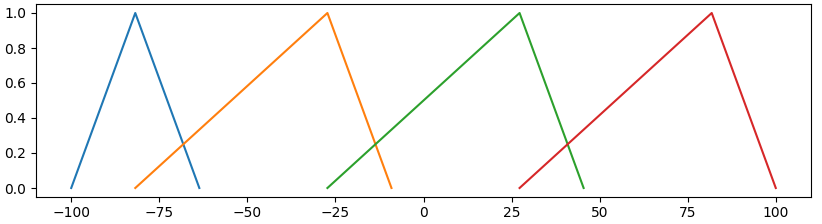
\includegraphics{mf_with_parameters.png}
\caption{Membership functions}
\end{figure}

Die Anordnung ist gleich bei allen Mengen außer die Erste. Damit keine
Definitionslücken entstehen, verzichte ich auf die Trainierung der
beiden Grenzwertparametern. Neben dem Trainingsausschluß des ersten
Parameter der ersten Menge und des letzten der letzen Mengen, die die
Wertebereich bestimmen, werden auch weitere Einschränkungen angelegt.
Zum einen wird der Wert der Spitzenparameter(mittlerer Parameter) jeder
Funktion begrenzt, sodass er nicht kleiner als der linke Parameter, bzw.
größer als der rechte Parameter, wird. Ohne diese Regel entstehen
manchmal ungültige Fuzzy-Mengen.

Infolge des Austesten tauchten kritischen Fehler bezüglich der
Undefiniertheit der Zugehörigkeitsfunktionen auf. Diese Mangeln könnte
ich mit drei Einschränkungen aufheben. Die Beschränkungen fallen auf die
drei Parametern, \(\textit{a, m, b}\), genauer gesagt die
Dreiecksfunktionsparameter:

%    \begin{Verbatim}[commandchars=\\\{\}]
%{\color{incolor}In [{\color{incolor} }]:} \PY{c+c1}{\PYZsh{} ...}
%        \PY{n+nb+bp}{self}\PY{o}{.}\PY{n}{constraints}\PY{o}{.}\PY{n}{append}\PY{p}{(}\PY{n}{tf}\PY{o}{.}\PY{n}{assign}\PY{p}{(}\PY{n}{a}\PY{p}{,} \PY{n}{tf}\PY{o}{.}\PY{n}{clip\PYZus{}by\PYZus{}value}\PY{p}{(}\PY{n}{a}\PY{p}{,} \PY{n+nb+bp}{self}\PY{o}{.}\PY{n}{range}\PY{p}{[}\PY{l+m+mi}{0}\PY{p}{]}\PY{p}{,} \PY{n}{m} \PY{o}{\PYZhy{}} \PY{l+m+mf}{1e\PYZhy{}2}\PY{p}{)}\PY{p}{)}\PY{p}{)}
%        \PY{n+nb+bp}{self}\PY{o}{.}\PY{n}{constraints}\PY{o}{.}\PY{n}{append}\PY{p}{(}\PY{n}{tf}\PY{o}{.}\PY{n}{assign}\PY{p}{(}\PY{n}{b}\PY{p}{,} \PY{n}{tf}\PY{o}{.}\PY{n}{clip\PYZus{}by\PYZus{}value}\PY{p}{(}\PY{n}{b}\PY{p}{,} \PY{n}{m} \PY{o}{+} \PY{l+m+mf}{1e\PYZhy{}2}\PY{p}{,} \PY{n+nb+bp}{self}\PY{o}{.}\PY{n}{range}\PY{p}{[}\PY{l+m+mi}{1}\PY{p}{]}\PY{p}{)}\PY{p}{)}\PY{p}{)}
%        \PY{n+nb+bp}{self}\PY{o}{.}\PY{n}{constraints}\PY{o}{.}\PY{n}{append}\PY{p}{(}\PY{n}{tf}\PY{o}{.}\PY{n}{assign}\PY{p}{(}\PY{n}{m}\PY{p}{,} \PY{n}{tf}\PY{o}{.}\PY{n}{clip\PYZus{}by\PYZus{}value}\PY{p}{(}\PY{n}{m}\PY{p}{,} \PY{n+nb+bp}{self}\PY{o}{.}\PY{n}{range}\PY{p}{[}\PY{l+m+mi}{0}\PY{p}{]} \PY{o}{+} \PY{l+m+mf}{0.1}\PY{p}{,} \PY{n+nb+bp}{self}\PY{o}{.}\PY{n}{range}\PY{p}{[}\PY{l+m+mi}{1}\PY{p}{]} \PY{o}{\PYZhy{}} \PY{l+m+mf}{0.1}\PY{p}{)}\PY{p}{)}\PY{p}{)}
%        \PY{c+c1}{\PYZsh{} ...}
%\end{Verbatim}

    \hypertarget{zweiter-programmteil-third-layer}{%
\subsubsection{Zweiter Programmteil (Third
Layer)}\label{zweiter-programmteil-third-layer}}

Der zweite Programmteil enthält weniger Programmcode, aber dauert unter
Umständen länger. Die lange Laufzeit ergibt sich aus der Berechnung der
Permutationen der ZGF für alle Eingaben. Die Bibliothek
\(\textit{itertools}\) stellt mehrer Funktion bereit. Eine der Methoden
daraus berechnet das kartesische Produkt. Die Funktion kann mehrere
Mengen und einen \textbf{repeat}-Parameter entgegennehmen und liefert
eine Ergebnismenge. Die \textbf{repeat}-Variable gibt an, wie oft das
kartesische Produkt ausgeführt wird. Die Iteratorfunktion ist in der
Komplexitätsklasse \(TIME_{product()} \in O(n^k)\), mit \emph{n} gleich
die Anzahl der Elemente in der Angegebene Menge und \emph{k} gleich die
Anzahl der Ausführungen. Ein kleines Beispiel zur Verdeutlichung als
auch eine Implementierung des zweiten Programmteils wird unten gegeben.

%    \begin{Verbatim}[commandchars=\\\{\}]
%{\color{incolor}In [{\color{incolor}5}]:} \PY{c+c1}{\PYZsh{} itertools.product(l, r) builds the cartesian product of the iterables (the list l).}
%        \PY{c+c1}{\PYZsh{} if r is equal to two, this would return the cartesian product of the list l with itself (l x l).}
%        \PY{c+c1}{\PYZsh{} if r is three \PYZhy{} (l x l x l). We use it here to get all the combinations between the inputs}
%        \PY{c+c1}{\PYZsh{} Example: product((A, B), repeat=2) would result in the list [(A, A), (A, B), (B, A), (B, B)]}
%        \PY{k}{for} \PY{n}{perm} \PY{o+ow}{in} \PY{n}{it}\PY{o}{.}\PY{n}{product}\PY{p}{(}\PY{n+nb}{range}\PY{p}{(}\PY{n+nb+bp}{self}\PY{o}{.}\PY{n}{num\PYZus{}sets}\PY{p}{)}\PY{p}{,} \PY{n}{repeat}\PY{o}{=}\PY{n+nb+bp}{self}\PY{o}{.}\PY{n}{num\PYZus{}inputs}\PY{p}{)}\PY{p}{:}
%            \PY{n}{tmp} \PY{o}{=} \PY{n}{tf}\PY{o}{.}\PY{n}{ones}\PY{p}{(}\PY{n}{shape}\PY{o}{=}\PY{p}{(}\PY{p}{)}\PY{p}{,} \PY{n}{dtype}\PY{o}{=}\PY{n}{tf}\PY{o}{.}\PY{n}{float64}\PY{p}{)}
%            \PY{c+c1}{\PYZsh{} loop from 0 to self.num\PYZus{}inputs and multiply the MF of an input with index perm[i] with}
%            \PY{c+c1}{\PYZsh{} every other MF with index from the permutation list}
%            \PY{k}{for} \PY{n}{i} \PY{o+ow}{in} \PY{n+nb}{range}\PY{p}{(}\PY{n+nb}{len}\PY{p}{(}\PY{n}{perm}\PY{p}{)}\PY{p}{)}\PY{p}{:}
%                \PY{n}{tmp} \PY{o}{=} \PY{n}{tf}\PY{o}{.}\PY{n}{multiply}\PY{p}{(}\PY{n}{premises}\PY{p}{[}\PY{n}{i}\PY{p}{]}\PY{p}{[}\PY{n}{perm}\PY{p}{[}\PY{n}{i}\PY{p}{]}\PY{p}{]}\PY{p}{,} \PY{n}{tmp}\PY{p}{)}
%            \PY{n+nb+bp}{self}\PY{o}{.}\PY{n}{mf}\PY{p}{[}\PY{n}{index}\PY{p}{]} \PY{o}{=} \PY{n}{tmp}
%            \PY{n}{index} \PY{o}{+}\PY{o}{=} \PY{l+m+mi}{1}
%        \PY{n}{end} \PY{o}{=} \PY{n}{t}\PY{o}{.}\PY{n}{process\PYZus{}time}\PY{p}{(}\PY{p}{)}
%        \PY{n+nb}{print}\PY{p}{(}\PY{l+s+s2}{\PYZdq{}}\PY{l+s+s2}{Initializing all the Permutation took }\PY{l+s+si}{\PYZpc{}f}\PY{l+s+s2}{ s}\PY{l+s+s2}{\PYZdq{}} \PY{o}{\PYZpc{}} \PY{p}{(}\PY{n}{end} \PY{o}{\PYZhy{}} \PY{n}{start}\PY{p}{)}\PY{p}{)}
%\end{Verbatim}
%
%    \begin{Verbatim}[commandchars=\\\{\}]
%
%          File "<ipython-input-5-82dd3365547d>", line 2
%        start = t.process\_time()
%        \^{}
%    IndentationError: unexpected indent
%
%
%    \end{Verbatim}

    Aus der Komplexitätsklasse ergibt sich, wie oft die äußere Schleife
ausgeführt wird. Genauer gesagt, der Loop braucht so viele Iterationen
bis zum Schluss wie die Gesamtzahl der Regeln. In der innere Schleife
werden die Elemente in der Liste durchlaufen. Pro Iteration wird ein
Element aus der Productliste betrachtet. Jeder Eintrag aus der Liste
repräsentiert ein Index \textbf{perm{[}i{]}} einer
Zugehörigkeitsfunktion für die entsprechende Eingabe \textbf{i}. Die
Funktionen werden der Reihe nach mit einem Dummy-Tensor multiplizert.
Auf dieser Weise werden die Prämisse jeder Regel definiert.

    \hypertarget{fourth-layer}{%
\subsubsection{Fourth Layer}\label{fourth-layer}}

Im dritten Layer laut der Struktur des ANFIS-Models, werden alle
Ergebnisse aus dem vorrigen Schicht normiert. Die Funktion besteht nur
aus zwei Zeilen Code:

%    \begin{Verbatim}[commandchars=\\\{\}]
%{\color{incolor}In [{\color{incolor} }]:} \PY{k}{def} \PY{n+nf}{third\PYZus{}layer}\PY{p}{(}\PY{n+nb+bp}{self}\PY{p}{)}\PY{p}{:}
%            \PY{c+c1}{\PYZsh{} Reshape the MFs}
%            \PY{c+c1}{\PYZsh{} Reshape the array, to be in the form of an array with num\PYZus{}rules items in it}
%            \PY{c+c1}{\PYZsh{} sum the elements in the array along the 0th dimension}
%            \PY{n+nb+bp}{self}\PY{o}{.}\PY{n}{mf\PYZus{}sum} \PY{o}{=} \PY{n}{tf}\PY{o}{.}\PY{n}{reduce\PYZus{}sum}\PY{p}{(}\PY{n}{tf}\PY{o}{.}\PY{n}{add}\PY{p}{(}\PY{n+nb+bp}{self}\PY{o}{.}\PY{n}{mf}\PY{p}{,} \PY{p}{[}\PY{l+m+mf}{1e\PYZhy{}10}\PY{p}{]}\PY{p}{)}\PY{p}{,} \PY{l+m+mi}{0}\PY{p}{)}
%            \PY{c+c1}{\PYZsh{} Normalize the MFs}
%            \PY{c+c1}{\PYZsh{} Add all the items in the vector and divide every item in it with the sum of the elements}
%            \PY{c+c1}{\PYZsh{} This way we get the normalized membership functions}
%            \PY{n+nb+bp}{self}\PY{o}{.}\PY{n}{normalizedMFs} \PY{o}{=} \PY{n}{tf}\PY{o}{.}\PY{n}{divide}\PY{p}{(}\PY{n+nb+bp}{self}\PY{o}{.}\PY{n}{mf}\PY{p}{,} \PY{n+nb+bp}{self}\PY{o}{.}\PY{n}{mf\PYZus{}sum}\PY{p}{)}
%\end{Verbatim}

    Mit der Funktion \textbf{reduce\_sum()} werden die Einträge in einem
Array, bzw. Matrix oder Vektor, zusammensumiert. Es kann einen
zusätzlichen Parameter angegeben werden, der in der Dokumentation als
\textbf{axis} beschriftet ist und der angibt, welche Achse entlang die
Elemente summiert werden sollen. Wie man am oberen Programmcode erkennt,
werden hier die Elemente die 0. Achse entlang summiert. Wenn wir eine
Matrix betrachten würden, heißt das für die Summe, dass die Elemente in
einer Spalte summiert werden. Das Ergebnis der Summierung wird
entsprechend in einer Variable abgespeichert, da wir einen
zwei-Dimensionalen Array mit jeweils einen Eintrag in der zweite
Dimension, erhalten wir eine Zahl. Schließlich werden alle
Zugehörigkeitsfunktionen durch diesen Wert geteilt. Auf diesem Weg wird
das Ergebnis der Prämissen normiert und ihre Summe gleich \emph{1}.

\hypertarget{fifth-layer}{%
\subsubsection{Fifth Layer}\label{fifth-layer}}

Die fünfte Schicht soll das Ergebnis aus jeder Konklusionsfunktion
berechnen. Die Ausgabe erhalten wird, in dem die Eingangsgrößen in jeden
Konklusionsfunktion eingesetzt werden und der Zutriffswert der Regeln an
dem Funktionswert multipliziert werden. Durch die Normalisierung der
Eintretungsgrößen erhalten wir eine Summe der Gewichte von 1, also ein
Ergebnis mit Faktor kleiner 1 wird ausgegeben.

%    \begin{Verbatim}[commandchars=\\\{\}]
%{\color{incolor}In [{\color{incolor} }]:} \PY{k}{def} \PY{n+nf}{fifth\PYZus{}layer}\PY{p}{(}\PY{n+nb+bp}{self}\PY{p}{)}\PY{p}{:}
%            \PY{c+c1}{\PYZsh{} multiply every premis with its coresponding conclusion function}
%            \PY{c+c1}{\PYZsh{} we get a vektor of results with each result having a factor less than 1}
%            \PY{n+nb+bp}{self}\PY{o}{.}\PY{n}{outputs} \PY{o}{=} \PY{n}{tf}\PY{o}{.}\PY{n}{multiply}\PY{p}{(}\PY{n+nb+bp}{self}\PY{o}{.}\PY{n}{normalizedMFs}\PY{p}{,} \PY{n+nb+bp}{self}\PY{o}{.}\PY{n}{conclusions}\PY{p}{)}
%\end{Verbatim}

    \hypertarget{sixth-layer}{%
\subsubsection{Sixth Layer}\label{sixth-layer}}

Die Summe aller Werten und das eigentliche Ergebnis für ein gegebenes
Kandidat \textbf{X} wird in der letzen (sechsten) Schicht berechnet.
Dies erfolgt in einem Einzeiler:

%    \begin{Verbatim}[commandchars=\\\{\}]
%{\color{incolor}In [{\color{incolor} }]:} \PY{k}{def} \PY{n+nf}{sixth\PYZus{}layer}\PY{p}{(}\PY{n+nb+bp}{self}\PY{p}{)}\PY{p}{:}
%            \PY{n+nb+bp}{self}\PY{o}{.}\PY{n}{result} \PY{o}{=} \PY{n}{tf}\PY{o}{.}\PY{n}{reduce\PYZus{}sum}\PY{p}{(}\PY{n+nb+bp}{self}\PY{o}{.}\PY{n}{outputs}\PY{p}{,} \PY{l+m+mi}{0}\PY{p}{)}
%\end{Verbatim}

    \hypertarget{optimisierungsfunktion}{%
\subsection{Optimisierungsfunktion}\label{optimisierungsfunktion}}

Nachdem das Neuronale Model aufgebaut wird, folgt die Definition des
Optimierungsverfahren. In der Literatur, auch in der Praxis, wird die
Kleinste-Quadrate Funktion verwendet. Auch hier habe ich diese
eingesetzt. Als nächstes muss der Optimiser definiert werden. Die zwei
bekanntesten sind \emph{GradientDescnetOptimizer} und
\emph{AdamOptimizer}. Bei der Auswahl gibt es keinen klaren besseren
Algorithmus. Um den richtigen Optimisierer auszuwählen, muss man mit den
unterschiedlichen Algorithmen gespielt haben, bis der Beste gefunden
wird. In meinem Fall ist der AdamOptimizer besser geeignet. Unten ist
die Definition der Funktion gegeben.

%    \begin{Verbatim}[commandchars=\\\{\}]
%{\color{incolor}In [{\color{incolor} }]:} \PY{k}{def} \PY{n+nf}{optimize\PYZus{}method}\PY{p}{(}\PY{n+nb+bp}{self}\PY{p}{)}\PY{p}{:}
%                \PY{n+nb+bp}{self}\PY{o}{.}\PY{n}{loss} \PY{o}{=} \PY{n}{tf}\PY{o}{.}\PY{n}{losses}\PY{o}{.}\PY{n}{mean\PYZus{}squared\PYZus{}error}\PY{p}{(}\PY{n+nb+bp}{self}\PY{o}{.}\PY{n}{y}\PY{p}{,} \PY{n+nb+bp}{self}\PY{o}{.}\PY{n}{result}\PY{p}{)}
%                \PY{c+c1}{\PYZsh{} self.loss = tf.losses.huber\PYZus{}loss(self.y, self.result)}
%        
%                \PY{c+c1}{\PYZsh{} self.optimizer = tf.train.GradientDescentOptimizer(learning\PYZus{}rate=0.01).minimize(self.loss)}
%                \PY{n+nb+bp}{self}\PY{o}{.}\PY{n}{optimizer} \PY{o}{=} \PY{n}{tf}\PY{o}{.}\PY{n}{train}\PY{o}{.}\PY{n}{AdamOptimizer}\PY{p}{(}\PY{n}{learning\PYZus{}rate}\PY{o}{=}\PY{l+m+mf}{0.1}\PY{p}{)}\PY{o}{.}\PY{n}{minimize}\PY{p}{(}\PY{n+nb+bp}{self}\PY{o}{.}\PY{n}{loss}\PY{p}{)}
%                \PY{c+c1}{\PYZsh{} self.optimizer = tf.train.RMSPropOptimizer(learning\PYZus{}rate=0.1).minimize(self.loss)}
%\end{Verbatim}

    Wie üblich die Fehlerate ergibt sich aus dem Soll- und Istergebnis.
Weiterhin erhalten wir den Optimierer durch einen simplen Codeaufruf,
während dessen auch einen Lernrate gegeben wird. Normalerweise wird die
Lernrate mit einem Wert von 0.1 gesetzt.

\hypertarget{trainingsfunktion}{%
\subsection{Trainingsfunktion}\label{trainingsfunktion}}

Mit den oben erklärten Funktionen kann einen ANFIS-Model mit beliebigen
Eigenschaften erstellt werden. Nach dem Ausbau folgt das eigentliche
Lernen. Darum habe ich eine separate Methode definiert, die den Ablauf
beim Lernen beschreibt.

%    \begin{Verbatim}[commandchars=\\\{\}]
%{\color{incolor}In [{\color{incolor} }]:}     \PY{k}{def} \PY{n+nf}{train}\PY{p}{(}\PY{n+nb+bp}{self}\PY{p}{,} \PY{n}{sess}\PY{p}{,} \PY{n}{epochs}\PY{o}{=}\PY{l+m+mi}{1}\PY{p}{)}\PY{p}{:}
%                \PY{c+c1}{\PYZsh{} first we init all the variables}
%                \PY{n}{sess}\PY{o}{.}\PY{n}{run}\PY{p}{(}\PY{n+nb+bp}{self}\PY{o}{.}\PY{n}{get\PYZus{}variable\PYZus{}initializer}\PY{p}{(}\PY{p}{)}\PY{p}{)}
%        
%                \PY{c+c1}{\PYZsh{} Init of arrays}
%                \PY{n}{x\PYZus{}val} \PY{o}{=} \PY{p}{[}\PY{p}{]}
%                \PY{n}{y\PYZus{}val} \PY{o}{=} \PY{p}{[}\PY{p}{]}
%                \PY{n}{y\PYZus{}before\PYZus{}trn} \PY{o}{=} \PY{p}{[}\PY{p}{]}
%                \PY{n}{y\PYZus{}after\PYZus{}trn} \PY{o}{=} \PY{p}{[}\PY{p}{]}
%        
%                \PY{c+c1}{\PYZsh{} Function before training}
%                \PY{c+c1}{\PYZsh{} we create a plot with num\PYZus{}inputs*2 + 1 subplots}
%                \PY{c+c1}{\PYZsh{} two subplots for every input. one sub is for the mfs before and one after the training}
%                \PY{n}{fig}\PY{p}{,} \PY{n}{axs} \PY{o}{=} \PY{n}{plt}\PY{o}{.}\PY{n}{subplots}\PY{p}{(}\PY{n+nb+bp}{self}\PY{o}{.}\PY{n}{num\PYZus{}inputs} \PY{o}{*} \PY{l+m+mi}{2} \PY{o}{+} \PY{l+m+mi}{1}\PY{p}{,} \PY{l+m+mi}{1}\PY{p}{,} \PY{n}{figsize}\PY{o}{=}\PY{p}{(}\PY{l+m+mi}{10}\PY{p}{,} \PY{l+m+mi}{9}\PY{p}{)}\PY{p}{)}
%                \PY{n}{plt}\PY{o}{.}\PY{n}{subplots\PYZus{}adjust}\PY{p}{(}\PY{n}{top}\PY{o}{=}\PY{l+m+mf}{0.88}\PY{p}{,} \PY{n}{hspace}\PY{o}{=}\PY{l+m+mf}{0.3}\PY{p}{)}
%                
%                \PY{c+c1}{\PYZsh{} We plot the mfs in the upper subplot}
%                \PY{k}{for} \PY{n}{i} \PY{o+ow}{in} \PY{n+nb}{range}\PY{p}{(}\PY{n+nb+bp}{self}\PY{o}{.}\PY{n}{num\PYZus{}inputs}\PY{p}{)}\PY{p}{:}
%                    \PY{n+nb}{vars} \PY{o}{=} \PY{n+nb+bp}{self}\PY{o}{.}\PY{n}{plot\PYZus{}param}\PY{p}{(}\PY{n}{sess}\PY{p}{,} \PY{n}{axs}\PY{p}{[}\PY{n}{i} \PY{o}{+} \PY{l+m+mi}{1}\PY{p}{]}\PY{p}{,}
%                                           \PY{l+s+s2}{\PYZdq{}}\PY{l+s+s2}{MF }\PY{l+s+si}{\PYZpc{}d}\PY{l+s+s2}{ before training}\PY{l+s+s2}{\PYZdq{}} \PY{o}{\PYZpc{}} \PY{p}{(}\PY{n}{i} \PY{o}{+} \PY{l+m+mi}{1}\PY{p}{)}\PY{p}{)}
%                    \PY{n+nb}{print}\PY{p}{(}\PY{l+s+s2}{\PYZdq{}}\PY{l+s+s2}{Parameters vor dem Training: }\PY{l+s+si}{\PYZob{}\PYZcb{}}\PY{l+s+s2}{ }\PY{l+s+se}{\PYZbs{}n}\PY{l+s+s2}{\PYZdq{}}\PY{o}{.}\PY{n}{format}\PY{p}{(}\PY{n+nb}{vars}\PY{p}{[}\PY{n}{i}\PY{p}{]}\PY{p}{)}\PY{p}{)}
%                
%                \PY{c+c1}{\PYZsh{} depending on the gradient type we do three types of calculating the test result}
%                \PY{c+c1}{\PYZsh{} first one is the stochastic gradient descent}
%                \PY{c+c1}{\PYZsh{} we calculate the result for each item in the data}
%                \PY{k}{if} \PY{n+nb+bp}{self}\PY{o}{.}\PY{n}{gradient\PYZus{}type} \PY{o}{==} \PY{l+m+mi}{0}\PY{p}{:}
%                    \PY{k}{for} \PY{n}{i} \PY{o+ow}{in} \PY{n+nb}{range}\PY{p}{(}\PY{n+nb}{len}\PY{p}{(}\PY{n+nb+bp}{self}\PY{o}{.}\PY{n}{test\PYZus{}x\PYZus{}arr}\PY{p}{)}\PY{p}{)}\PY{p}{:}
%                        \PY{n}{arr\PYZus{}x} \PY{o}{=} \PY{n+nb+bp}{self}\PY{o}{.}\PY{n}{test\PYZus{}x\PYZus{}arr}\PY{p}{[}\PY{n}{i}\PY{p}{]}
%                        \PY{n}{arr\PYZus{}y} \PY{o}{=} \PY{n+nb+bp}{self}\PY{o}{.}\PY{n}{test\PYZus{}y\PYZus{}arr}\PY{p}{[}\PY{n}{i}\PY{p}{]}
%                        \PY{n}{x\PYZus{}val}\PY{o}{.}\PY{n}{append}\PY{p}{(}\PY{n+nb+bp}{self}\PY{o}{.}\PY{n}{test\PYZus{}x\PYZus{}arr}\PY{p}{[}\PY{n}{i}\PY{p}{]}\PY{p}{[}\PY{l+m+mi}{0}\PY{p}{]}\PY{p}{)}
%                        \PY{n}{y\PYZus{}val}\PY{o}{.}\PY{n}{append}\PY{p}{(}\PY{n+nb+bp}{self}\PY{o}{.}\PY{n}{test\PYZus{}y\PYZus{}arr}\PY{p}{[}\PY{n}{i}\PY{p}{]}\PY{p}{[}\PY{l+m+mi}{0}\PY{p}{]}\PY{p}{)}
%        
%                        \PY{n}{y\PYZus{}before\PYZus{}trn}\PY{o}{.}\PY{n}{append}\PY{p}{(}\PY{n+nb+bp}{self}\PY{o}{.}\PY{n}{do\PYZus{}calculation}\PY{p}{(}\PY{n}{sess}\PY{p}{,} \PY{n+nb+bp}{self}\PY{o}{.}\PY{n}{test\PYZus{}x\PYZus{}arr}\PY{p}{[}\PY{n}{i}\PY{p}{]}\PY{p}{)}\PY{p}{)}
%                \PY{c+c1}{\PYZsh{} here the gradient type is set to two}
%                \PY{c+c1}{\PYZsh{} so we calculate the result with the whole data set}
%                \PY{k}{elif} \PY{n+nb+bp}{self}\PY{o}{.}\PY{n}{gradient\PYZus{}type} \PY{o}{==} \PY{l+m+mi}{2}\PY{p}{:}
%                    \PY{n}{x\PYZus{}val} \PY{o}{=} \PY{n}{np}\PY{o}{.}\PY{n}{reshape}\PY{p}{(}\PY{n+nb+bp}{self}\PY{o}{.}\PY{n}{test\PYZus{}x\PYZus{}arr}\PY{p}{,} \PY{p}{(}\PY{n+nb}{len}\PY{p}{(}\PY{n+nb+bp}{self}\PY{o}{.}\PY{n}{test\PYZus{}x\PYZus{}arr}\PY{p}{)}\PY{p}{)}\PY{p}{)}
%                    \PY{n}{y\PYZus{}val} \PY{o}{=} \PY{n}{np}\PY{o}{.}\PY{n}{reshape}\PY{p}{(}\PY{n+nb+bp}{self}\PY{o}{.}\PY{n}{test\PYZus{}y\PYZus{}arr}\PY{p}{,} \PY{p}{(}\PY{n+nb}{len}\PY{p}{(}\PY{n+nb+bp}{self}\PY{o}{.}\PY{n}{test\PYZus{}x\PYZus{}arr}\PY{p}{)}\PY{p}{)}\PY{p}{)}
%        
%                    \PY{n}{y\PYZus{}before\PYZus{}trn} \PY{o}{=} \PY{n+nb+bp}{self}\PY{o}{.}\PY{n}{do\PYZus{}calculation}\PY{p}{(}\PY{n}{sess}\PY{p}{,} \PY{n}{x\PYZus{}val}\PY{p}{)}
%                \PY{c+c1}{\PYZsh{} finally if we have set the type to 1 we calculate for a fraction of the whole set}
%                \PY{c+c1}{\PYZsh{} usually we do 1/5 of the whole set, because i use data wich ends with a 0, }
%                \PY{c+c1}{\PYZsh{} so it is dividable by 5 with no rest}
%                \PY{k}{else}\PY{p}{:}
%                    \PY{k}{for} \PY{n}{i} \PY{o+ow}{in} \PY{n+nb}{range}\PY{p}{(}\PY{l+m+mi}{5}\PY{p}{)}\PY{p}{:}
%                        \PY{n}{start\PYZus{}index} \PY{o}{=} \PY{n}{i} \PY{o}{*} \PY{n+nb+bp}{self}\PY{o}{.}\PY{n}{mini\PYZus{}batch\PYZus{}size}
%                        \PY{n}{end\PYZus{}index} \PY{o}{=} \PY{p}{(}\PY{n}{i} \PY{o}{+} \PY{l+m+mi}{1}\PY{p}{)} \PY{o}{*} \PY{n+nb+bp}{self}\PY{o}{.}\PY{n}{mini\PYZus{}batch\PYZus{}size}
%        
%                        \PY{n}{arr\PYZus{}x} \PY{o}{=} \PY{n+nb+bp}{self}\PY{o}{.}\PY{n}{test\PYZus{}x\PYZus{}arr}\PY{p}{[}\PY{n}{start\PYZus{}index}\PY{p}{:}\PY{n}{end\PYZus{}index}\PY{p}{]}
%                        \PY{n}{arr\PYZus{}y} \PY{o}{=} \PY{n+nb+bp}{self}\PY{o}{.}\PY{n}{test\PYZus{}y\PYZus{}arr}\PY{p}{[}\PY{n}{start\PYZus{}index}\PY{p}{:}\PY{n}{end\PYZus{}index}\PY{p}{]}
%                        \PY{n}{arr\PYZus{}x} \PY{o}{=} \PY{n}{np}\PY{o}{.}\PY{n}{reshape}\PY{p}{(}\PY{n}{arr\PYZus{}x}\PY{p}{,} \PY{p}{(}\PY{n+nb+bp}{self}\PY{o}{.}\PY{n}{mini\PYZus{}batch\PYZus{}size}\PY{p}{)}\PY{p}{)}
%        
%                        \PY{n}{x\PYZus{}val}\PY{o}{.}\PY{n}{append}\PY{p}{(}\PY{n}{arr\PYZus{}x}\PY{p}{)}
%                        \PY{n}{y\PYZus{}val}\PY{o}{.}\PY{n}{append}\PY{p}{(}\PY{n}{arr\PYZus{}y}\PY{p}{)}
%        
%                        \PY{n}{y\PYZus{}before\PYZus{}trn}\PY{o}{.}\PY{n}{append}\PY{p}{(}\PY{n+nb+bp}{self}\PY{o}{.}\PY{n}{do\PYZus{}calculation}\PY{p}{(}\PY{n}{sess}\PY{p}{,} \PY{n}{arr\PYZus{}x}\PY{p}{)}\PY{p}{)}
%                
%                \PY{c+c1}{\PYZsh{} we reshape the arrays so it fits the input into the plot function}
%                \PY{n}{size} \PY{o}{=} \PY{n+nb}{len}\PY{p}{(}\PY{n+nb+bp}{self}\PY{o}{.}\PY{n}{test\PYZus{}x\PYZus{}arr}\PY{p}{)}
%                \PY{n}{x\PYZus{}val} \PY{o}{=} \PY{n}{np}\PY{o}{.}\PY{n}{reshape}\PY{p}{(}\PY{n}{x\PYZus{}val}\PY{p}{,} \PY{p}{(}\PY{n}{size}\PY{p}{)}\PY{p}{)}
%                \PY{n}{y\PYZus{}val} \PY{o}{=} \PY{n}{np}\PY{o}{.}\PY{n}{reshape}\PY{p}{(}\PY{n}{y\PYZus{}val}\PY{p}{,} \PY{p}{(}\PY{n}{size}\PY{p}{)}\PY{p}{)}
%                \PY{n}{y\PYZus{}before\PYZus{}trn} \PY{o}{=} \PY{n}{np}\PY{o}{.}\PY{n}{reshape}\PY{p}{(}\PY{n}{y\PYZus{}before\PYZus{}trn}\PY{p}{,} \PY{p}{(}\PY{n}{size}\PY{p}{)}\PY{p}{)}
%            
%                \PY{n}{axs}\PY{p}{[}\PY{l+m+mi}{0}\PY{p}{]}\PY{o}{.}\PY{n}{plot}\PY{p}{(}\PY{n}{x\PYZus{}val}\PY{p}{,} \PY{n}{y\PYZus{}val}\PY{p}{,} \PY{n}{color}\PY{o}{=}\PY{l+s+s2}{\PYZdq{}}\PY{l+s+s2}{blue}\PY{l+s+s2}{\PYZdq{}}\PY{p}{)}
%                \PY{n}{axs}\PY{p}{[}\PY{l+m+mi}{0}\PY{p}{]}\PY{o}{.}\PY{n}{plot}\PY{p}{(}\PY{n}{x\PYZus{}val}\PY{p}{,} \PY{n}{y\PYZus{}before\PYZus{}trn}\PY{p}{,} \PY{n}{color}\PY{o}{=}\PY{l+s+s2}{\PYZdq{}}\PY{l+s+s2}{green}\PY{l+s+s2}{\PYZdq{}}\PY{p}{,} \PY{n}{alpha}\PY{o}{=}\PY{l+m+mf}{0.5}\PY{p}{)}
%        
%                \PY{c+c1}{\PYZsh{} Training Process}
%                \PY{c+c1}{\PYZsh{} we mesure the time it takes for the model the finish with the training}
%                \PY{c+c1}{\PYZsh{} analogical to the ploting, we have three types of learning}
%                \PY{n}{start} \PY{o}{=} \PY{n}{t}\PY{o}{.}\PY{n}{process\PYZus{}time}\PY{p}{(}\PY{p}{)}
%                \PY{k}{if} \PY{n+nb+bp}{self}\PY{o}{.}\PY{n}{gradient\PYZus{}type} \PY{o}{==} \PY{l+m+mi}{0}\PY{p}{:}
%                    \PY{k}{for} \PY{n}{s} \PY{o+ow}{in} \PY{n+nb}{range}\PY{p}{(}\PY{n}{epochs}\PY{p}{)}\PY{p}{:}
%                        \PY{k}{for} \PY{n}{i} \PY{o+ow}{in} \PY{n+nb}{range}\PY{p}{(}\PY{n+nb}{len}\PY{p}{(}\PY{n+nb+bp}{self}\PY{o}{.}\PY{n}{train\PYZus{}x\PYZus{}arr}\PY{p}{)}\PY{p}{)}\PY{p}{:}
%                            \PY{c+c1}{\PYZsh{} we run one iteration, when we run the optimizer function, after}
%                            \PY{c+c1}{\PYZsh{} at the end of every iteration we fit the parameters of the model}
%                            \PY{n}{sess}\PY{o}{.}\PY{n}{run}\PY{p}{(}\PY{p}{[}\PY{n+nb+bp}{self}\PY{o}{.}\PY{n}{loss}\PY{p}{,} \PY{n+nb+bp}{self}\PY{o}{.}\PY{n}{optimizer}\PY{p}{]}\PY{p}{,}
%                                     \PY{n}{feed\PYZus{}dict}\PY{o}{=}
%                                     \PY{p}{\PYZob{}}\PY{n+nb+bp}{self}\PY{o}{.}\PY{n}{x}\PY{p}{:} \PY{p}{[}\PY{n+nb+bp}{self}\PY{o}{.}\PY{n}{train\PYZus{}x\PYZus{}arr}\PY{p}{[}\PY{n}{i}\PY{p}{]}\PY{p}{]}\PY{p}{,} \PY{n+nb+bp}{self}\PY{o}{.}\PY{n}{y}\PY{p}{:} \PY{n+nb+bp}{self}\PY{o}{.}\PY{n}{train\PYZus{}y\PYZus{}arr}\PY{p}{[}\PY{n}{i}\PY{p}{]}\PY{p}{\PYZcb{}}\PY{p}{)}
%                            \PY{c+c1}{\PYZsh{} at the end we run all the constraints so we ensure there are no undefined ranges}
%                            \PY{n}{sess}\PY{o}{.}\PY{n}{run}\PY{p}{(}\PY{n+nb+bp}{self}\PY{o}{.}\PY{n}{constraints}\PY{p}{)}
%                \PY{k}{elif} \PY{n+nb+bp}{self}\PY{o}{.}\PY{n}{gradient\PYZus{}type} \PY{o}{==} \PY{l+m+mi}{1}\PY{p}{:}
%                    \PY{n}{times} \PY{o}{=} \PY{l+m+mi}{5}
%                    \PY{c+c1}{\PYZsh{} times = int(len(self.train\PYZus{}x\PYZus{}arr) / self.mini\PYZus{}batch\PYZus{}size)}
%                    \PY{k}{for} \PY{n}{i} \PY{o+ow}{in} \PY{n+nb}{range}\PY{p}{(}\PY{n}{epochs}\PY{p}{)}\PY{p}{:}
%                        \PY{k}{for} \PY{n}{j} \PY{o+ow}{in} \PY{n+nb}{range}\PY{p}{(}\PY{n}{times}\PY{p}{)}\PY{p}{:}
%                            \PY{n}{batch\PYZus{}x}\PY{p}{,} \PY{n}{batch\PYZus{}y} \PY{o}{=} \PY{n+nb+bp}{self}\PY{o}{.}\PY{n}{\PYZus{}\PYZus{}pick\PYZus{}batch}\PY{p}{(}\PY{p}{)}
%                            \PY{n}{batch\PYZus{}x} \PY{o}{=} \PY{n}{np}\PY{o}{.}\PY{n}{reshape}\PY{p}{(}\PY{n}{batch\PYZus{}x}\PY{p}{,} \PY{p}{(}\PY{n+nb+bp}{self}\PY{o}{.}\PY{n}{mini\PYZus{}batch\PYZus{}size}\PY{p}{)}\PY{p}{)}
%                            \PY{n}{batch\PYZus{}y} \PY{o}{=} \PY{n}{np}\PY{o}{.}\PY{n}{reshape}\PY{p}{(}\PY{n}{batch\PYZus{}y}\PY{p}{,} \PY{p}{(}\PY{n+nb+bp}{self}\PY{o}{.}\PY{n}{mini\PYZus{}batch\PYZus{}size}\PY{p}{)}\PY{p}{)}
%                            
%                            \PY{c+c1}{\PYZsh{} analog like type 0}
%                            \PY{n}{sess}\PY{o}{.}\PY{n}{run}\PY{p}{(}\PY{p}{[}\PY{n+nb+bp}{self}\PY{o}{.}\PY{n}{loss}\PY{p}{,} \PY{n+nb+bp}{self}\PY{o}{.}\PY{n}{optimizer}\PY{p}{]}\PY{p}{,}
%                                     \PY{n}{feed\PYZus{}dict}\PY{o}{=}\PY{p}{\PYZob{}}\PY{n+nb+bp}{self}\PY{o}{.}\PY{n}{x}\PY{p}{:} \PY{p}{[}\PY{n}{batch\PYZus{}x}\PY{p}{]}\PY{p}{,} \PY{n+nb+bp}{self}\PY{o}{.}\PY{n}{y}\PY{p}{:} \PY{n}{batch\PYZus{}y}\PY{p}{\PYZcb{}}\PY{p}{)}
%        
%                            \PY{n}{sess}\PY{o}{.}\PY{n}{run}\PY{p}{(}\PY{n+nb+bp}{self}\PY{o}{.}\PY{n}{constraints}\PY{p}{)}
%                \PY{k}{else}\PY{p}{:}
%                    \PY{k}{for} \PY{n}{i} \PY{o+ow}{in} \PY{n+nb}{range}\PY{p}{(}\PY{n}{epochs}\PY{p}{)}\PY{p}{:}
%                        \PY{n}{size} \PY{o}{=} \PY{n+nb}{len}\PY{p}{(}\PY{n+nb+bp}{self}\PY{o}{.}\PY{n}{train\PYZus{}x\PYZus{}arr}\PY{p}{)}
%                        \PY{n}{x\PYZus{}arr} \PY{o}{=} \PY{n}{np}\PY{o}{.}\PY{n}{reshape}\PY{p}{(}\PY{n+nb+bp}{self}\PY{o}{.}\PY{n}{train\PYZus{}x\PYZus{}arr}\PY{p}{,} \PY{p}{(}\PY{n}{size}\PY{p}{)}\PY{p}{)}
%                        \PY{n}{y\PYZus{}arr} \PY{o}{=} \PY{n}{np}\PY{o}{.}\PY{n}{reshape}\PY{p}{(}\PY{n+nb+bp}{self}\PY{o}{.}\PY{n}{train\PYZus{}y\PYZus{}arr}\PY{p}{,} \PY{p}{(}\PY{n}{size}\PY{p}{)}\PY{p}{)}
%                        \PY{c+c1}{\PYZsh{} analog like type 0}
%                        \PY{n}{sess}\PY{o}{.}\PY{n}{run}\PY{p}{(}\PY{p}{[}\PY{n+nb+bp}{self}\PY{o}{.}\PY{n}{loss}\PY{p}{,} \PY{n+nb+bp}{self}\PY{o}{.}\PY{n}{optimizer}\PY{p}{]}\PY{p}{,}
%                                 \PY{n}{feed\PYZus{}dict}\PY{o}{=}\PY{p}{\PYZob{}}\PY{n+nb+bp}{self}\PY{o}{.}\PY{n}{x}\PY{p}{:} \PY{n}{x\PYZus{}arr}\PY{p}{,} \PY{n+nb+bp}{self}\PY{o}{.}\PY{n}{y}\PY{p}{:} \PY{n}{y\PYZus{}arr}\PY{p}{\PYZcb{}}\PY{p}{)}
%                        \PY{n}{sess}\PY{o}{.}\PY{n}{run}\PY{p}{(}\PY{n+nb+bp}{self}\PY{o}{.}\PY{n}{constraints}\PY{p}{)}
%        
%                \PY{n}{end} \PY{o}{=} \PY{n}{t}\PY{o}{.}\PY{n}{process\PYZus{}time}\PY{p}{(}\PY{p}{)}
%                
%                \PY{c+c1}{\PYZsh{} then we fill our after training array with all the results}
%                \PY{k}{if} \PY{n+nb+bp}{self}\PY{o}{.}\PY{n}{gradient\PYZus{}type} \PY{o}{==} \PY{l+m+mi}{0}\PY{p}{:}
%                    \PY{k}{for} \PY{n}{i} \PY{o+ow}{in} \PY{n+nb}{range}\PY{p}{(}\PY{n+nb}{len}\PY{p}{(}\PY{n}{x\PYZus{}val}\PY{p}{)}\PY{p}{)}\PY{p}{:}
%                        \PY{n}{y\PYZus{}after\PYZus{}trn}\PY{o}{.}\PY{n}{append}\PY{p}{(}\PY{n+nb+bp}{self}\PY{o}{.}\PY{n}{do\PYZus{}calculation}\PY{p}{(}\PY{n}{sess}\PY{p}{,} \PY{n+nb+bp}{self}\PY{o}{.}\PY{n}{test\PYZus{}x\PYZus{}arr}\PY{p}{[}\PY{n}{i}\PY{p}{]}\PY{p}{)}\PY{p}{)}
%                \PY{k}{elif} \PY{n+nb+bp}{self}\PY{o}{.}\PY{n}{gradient\PYZus{}type} \PY{o}{==} \PY{l+m+mi}{1}\PY{p}{:}
%                    \PY{n}{times} \PY{o}{=} \PY{l+m+mi}{5}
%                    \PY{k}{for} \PY{n}{i} \PY{o+ow}{in} \PY{n+nb}{range}\PY{p}{(}\PY{n}{times}\PY{p}{)}\PY{p}{:}
%                        \PY{n}{start\PYZus{}index} \PY{o}{=} \PY{n}{i} \PY{o}{*} \PY{n+nb+bp}{self}\PY{o}{.}\PY{n}{mini\PYZus{}batch\PYZus{}size}
%                        \PY{n}{end\PYZus{}index} \PY{o}{=} \PY{p}{(}\PY{n}{i} \PY{o}{+} \PY{l+m+mi}{1}\PY{p}{)} \PY{o}{*} \PY{n+nb+bp}{self}\PY{o}{.}\PY{n}{mini\PYZus{}batch\PYZus{}size}
%        
%                        \PY{n}{arr\PYZus{}x} \PY{o}{=} \PY{n+nb+bp}{self}\PY{o}{.}\PY{n}{test\PYZus{}x\PYZus{}arr}\PY{p}{[}\PY{n}{start\PYZus{}index}\PY{p}{:}\PY{n}{end\PYZus{}index}\PY{p}{]}
%                        \PY{n}{arr\PYZus{}x} \PY{o}{=} \PY{n}{np}\PY{o}{.}\PY{n}{reshape}\PY{p}{(}\PY{n}{arr\PYZus{}x}\PY{p}{,} \PY{p}{(}\PY{n+nb+bp}{self}\PY{o}{.}\PY{n}{mini\PYZus{}batch\PYZus{}size}\PY{p}{)}\PY{p}{)}
%                        \PY{n}{y\PYZus{}after\PYZus{}trn}\PY{o}{.}\PY{n}{append}\PY{p}{(}\PY{n+nb+bp}{self}\PY{o}{.}\PY{n}{do\PYZus{}calculation}\PY{p}{(}\PY{n}{sess}\PY{p}{,} \PY{n}{arr\PYZus{}x}\PY{p}{)}\PY{p}{)}
%                \PY{k}{else}\PY{p}{:}
%                    \PY{n}{size} \PY{o}{=} \PY{n+nb}{len}\PY{p}{(}\PY{n+nb+bp}{self}\PY{o}{.}\PY{n}{test\PYZus{}x\PYZus{}arr}\PY{p}{)}
%                    \PY{n}{x\PYZus{}arr} \PY{o}{=} \PY{n}{np}\PY{o}{.}\PY{n}{reshape}\PY{p}{(}\PY{n+nb+bp}{self}\PY{o}{.}\PY{n}{test\PYZus{}x\PYZus{}arr}\PY{p}{,} \PY{p}{(}\PY{n}{size}\PY{p}{)}\PY{p}{)}
%                    \PY{n}{y\PYZus{}after\PYZus{}trn} \PY{o}{=} \PY{n+nb+bp}{self}\PY{o}{.}\PY{n}{do\PYZus{}calculation}\PY{p}{(}\PY{n}{sess}\PY{p}{,} \PY{n}{x\PYZus{}arr}\PY{p}{)}
%        
%                \PY{n}{size} \PY{o}{=} \PY{n+nb}{len}\PY{p}{(}\PY{n+nb+bp}{self}\PY{o}{.}\PY{n}{test\PYZus{}x\PYZus{}arr}\PY{p}{)}
%                \PY{n}{y\PYZus{}after\PYZus{}trn} \PY{o}{=} \PY{n}{np}\PY{o}{.}\PY{n}{reshape}\PY{p}{(}\PY{n}{y\PYZus{}after\PYZus{}trn}\PY{p}{,} \PY{p}{(}\PY{n}{size}\PY{p}{)}\PY{p}{)}
%        
%                \PY{c+c1}{\PYZsh{} Results after Training}
%                \PY{c+c1}{\PYZsh{} we plot the final graphic}
%                \PY{n}{axs}\PY{p}{[}\PY{l+m+mi}{0}\PY{p}{]}\PY{o}{.}\PY{n}{plot}\PY{p}{(}\PY{n+nb+bp}{self}\PY{o}{.}\PY{n}{test\PYZus{}x\PYZus{}arr}\PY{p}{,} \PY{n}{y\PYZus{}after\PYZus{}trn}\PY{p}{,} \PY{n}{color}\PY{o}{=}\PY{l+s+s1}{\PYZsq{}}\PY{l+s+s1}{red}\PY{l+s+s1}{\PYZsq{}}\PY{p}{,} \PY{n}{alpha}\PY{o}{=}\PY{l+m+mf}{0.5}\PY{p}{)}
%                
%                \PY{c+c1}{\PYZsh{} we set the labels on the subplot}
%                \PY{n}{axs}\PY{p}{[}\PY{l+m+mi}{0}\PY{p}{]}\PY{o}{.}\PY{n}{legend}\PY{p}{(}\PY{n}{bbox\PYZus{}to\PYZus{}anchor}\PY{o}{=}\PY{p}{(}\PY{l+m+mf}{0.}\PY{p}{,} \PY{l+m+mf}{1.02}\PY{p}{,} \PY{l+m+mf}{1.}\PY{p}{,} \PY{o}{.}\PY{l+m+mi}{102}\PY{p}{)}\PY{p}{,} \PY{n}{loc}\PY{o}{=}\PY{l+m+mi}{3}\PY{p}{,} \PY{n}{ncol}\PY{o}{=}\PY{l+m+mi}{1}\PY{p}{,}
%                              \PY{n}{mode}\PY{o}{=}\PY{l+s+s2}{\PYZdq{}}\PY{l+s+s2}{expand}\PY{l+s+s2}{\PYZdq{}}\PY{p}{,} \PY{n}{borderaxespad}\PY{o}{=}\PY{l+m+mf}{0.}\PY{p}{,}
%                              \PY{n}{labels}\PY{o}{=}\PY{p}{[}\PY{l+s+s2}{\PYZdq{}}\PY{l+s+s2}{Erwartete Werte}\PY{l+s+s2}{\PYZdq{}}\PY{p}{,} \PY{l+s+s2}{\PYZdq{}}\PY{l+s+s2}{Ergebnisse vor dem Training}\PY{l+s+s2}{\PYZdq{}}\PY{p}{,}
%                                      \PY{l+s+s2}{\PYZdq{}}\PY{l+s+s2}{Ergebnisse nach dem Training}\PY{l+s+s2}{\PYZdq{}}\PY{p}{]}\PY{p}{)}
%                \PY{c+c1}{\PYZsh{} and we plot the trained mf parameters}
%                \PY{k}{for} \PY{n}{i} \PY{o+ow}{in} \PY{n+nb}{range}\PY{p}{(}\PY{n+nb+bp}{self}\PY{o}{.}\PY{n}{num\PYZus{}inputs}\PY{p}{)}\PY{p}{:}
%                    \PY{n+nb}{vars} \PY{o}{=} \PY{n+nb+bp}{self}\PY{o}{.}\PY{n}{plot\PYZus{}param}\PY{p}{(}\PY{n}{sess}\PY{p}{,} \PY{n}{axs}\PY{p}{[}\PY{n+nb+bp}{self}\PY{o}{.}\PY{n}{num\PYZus{}inputs} \PY{o}{+} \PY{l+m+mi}{1} \PY{o}{+} \PY{n}{i}\PY{p}{]}\PY{p}{,}
%                                           \PY{l+s+s2}{\PYZdq{}}\PY{l+s+s2}{MF }\PY{l+s+si}{\PYZpc{}d}\PY{l+s+s2}{ after training}\PY{l+s+s2}{\PYZdq{}} \PY{o}{\PYZpc{}} \PY{p}{(}\PY{n}{i} \PY{o}{+} \PY{l+m+mi}{1}\PY{p}{)}\PY{p}{)}
%                    \PY{n+nb}{print}\PY{p}{(}\PY{l+s+s2}{\PYZdq{}}\PY{l+s+s2}{Parameters nach dem Training: }\PY{l+s+si}{\PYZob{}\PYZcb{}}\PY{l+s+s2}{ }\PY{l+s+se}{\PYZbs{}n}\PY{l+s+s2}{\PYZdq{}}\PY{o}{.}\PY{n}{format}\PY{p}{(}\PY{n+nb}{vars}\PY{p}{[}\PY{n}{i}\PY{p}{]}\PY{p}{)}\PY{p}{)}
%                
%                \PY{n}{prediction} \PY{o}{=} \PY{n}{y\PYZus{}after\PYZus{}trn}
%                \PY{n}{labels} \PY{o}{=} \PY{n}{y\PYZus{}val}
%                \PY{c+c1}{\PYZsh{} we calculate the error of the training}
%                \PY{n}{error} \PY{o}{=} \PY{n}{tf}\PY{o}{.}\PY{n}{losses}\PY{o}{.}\PY{n}{mean\PYZus{}squared\PYZus{}error}\PY{p}{(}\PY{n}{labels}\PY{p}{,} \PY{n}{prediction}\PY{p}{)}
%                \PY{n}{v} \PY{o}{=} \PY{n}{sess}\PY{o}{.}\PY{n}{run}\PY{p}{(}\PY{n}{error}\PY{p}{)}
%                \PY{n+nb}{print}\PY{p}{(}\PY{n}{v}\PY{p}{)}
%                
%                \PY{c+c1}{\PYZsh{} we construct the name of the training run}
%                \PY{n}{n} \PY{o}{=} \PY{n+nb+bp}{self}\PY{o}{.}\PY{n}{fileName} \PY{o}{+} \PY{l+s+s1}{\PYZsq{}}\PY{l+s+s1}{ 1 Input }\PY{l+s+s1}{\PYZsq{}} \PY{o}{+} \PY{n+nb}{str}\PY{p}{(}\PY{n+nb+bp}{self}\PY{o}{.}\PY{n}{num\PYZus{}sets}\PY{p}{)} \PY{o}{+} \PY{l+s+s1}{\PYZsq{}}\PY{l+s+s1}{ Sets }\PY{l+s+s1}{\PYZsq{}} \PY{o}{+} \PY{n+nb}{str}\PY{p}{(}\PY{n}{epochs}\PY{p}{)} \PY{o}{+} \PY{l+s+s1}{\PYZsq{}}\PY{l+s+s1}{ Epochs}\PY{l+s+s1}{\PYZsq{}}
%                
%                \PY{c+c1}{\PYZsh{} we save the plot to a file for later reference}
%                \PY{n}{fig}\PY{o}{.}\PY{n}{savefig}\PY{p}{(}\PY{l+s+s1}{\PYZsq{}}\PY{l+s+s1}{../graphics/fourthgraphics/}\PY{l+s+s1}{\PYZsq{}} \PY{o}{+}
%                            \PY{n}{n} \PY{o}{+} \PY{l+s+s1}{\PYZsq{}}\PY{l+s+s1}{.png}\PY{l+s+s1}{\PYZsq{}}\PY{p}{)}
%                
%                \PY{c+c1}{\PYZsh{} the gattered data is added to an array and saved into our .csv file}
%                \PY{n}{rowData} \PY{o}{=} \PY{p}{[}\PY{p}{[}\PY{n}{n}\PY{p}{,} \PY{n+nb}{str}\PY{p}{(}\PY{n}{end} \PY{o}{\PYZhy{}} \PY{n}{start}\PY{p}{)}\PY{p}{,} \PY{n+nb}{str}\PY{p}{(}\PY{n}{v}\PY{p}{)}\PY{p}{,} \PY{n}{gradient\PYZus{}types}\PY{p}{[}\PY{n+nb+bp}{self}\PY{o}{.}\PY{n}{gradient\PYZus{}type}\PY{p}{]}\PY{p}{]}\PY{p}{]}
%                \PY{n+nb}{print}\PY{p}{(}\PY{n}{rowData}\PY{p}{)}
%                \PY{n}{write\PYZus{}in\PYZus{}csv}\PY{p}{(}\PY{l+s+s1}{\PYZsq{}}\PY{l+s+s1}{../csvFiles/model\PYZus{}data.csv}\PY{l+s+s1}{\PYZsq{}}\PY{p}{,} \PY{n}{rowData}\PY{p}{)}
%                
%                \PY{c+c1}{\PYZsh{} we return the total amount of time it took to train the model}
%                \PY{k}{return} \PY{n}{end} \PY{o}{\PYZhy{}} \PY{n}{start}
%\end{Verbatim}

    Die Trainingsfunktion kann in vier Teile abgegrenzt werden. In dem
ersten Teil fallen alle Operationen für die Aufzeichnung der Grafiken
vor dem Lernen. Im zweiten Teil fällt der Lernzug. Danach kommt
entsprechend die Zeichnung der Änderungen des Models. Zum Schluss werden
alle Daten in Dateien abgespeichert.

\hypertarget{weitere-funktionen}{%
\subsection{Weitere Funktionen}\label{weitere-funktionen}}

In diesem Unterkapitel habe ich die zusätzlichen Funktionen angegeben.
Die sind weniger wichtig für das Verständnis des Programmablaufs. Eine
Erklärung dieser Funktionen wird in Kommentar unter dem Code gegeben.

%    \begin{Verbatim}[commandchars=\\\{\}]
%{\color{incolor}In [{\color{incolor} }]:}     \PY{k}{def} \PY{n+nf}{plot\PYZus{}param}\PY{p}{(}\PY{n+nb+bp}{self}\PY{p}{,} \PY{n}{sess}\PY{p}{,} \PY{n}{plot}\PY{p}{,} \PY{n}{name}\PY{p}{)}\PY{p}{:}
%                \PY{c+c1}{\PYZsh{} this function plots the mf parameters}
%                \PY{n}{mfpar} \PY{o}{=} \PY{n}{sess}\PY{o}{.}\PY{n}{run}\PY{p}{(}\PY{n+nb+bp}{self}\PY{o}{.}\PY{n}{var}\PY{p}{)}
%                \PY{n}{xArr} \PY{o}{=} \PY{p}{[}\PY{p}{]}
%                \PY{n}{yArr} \PY{o}{=} \PY{p}{[}\PY{p}{]}
%        
%                \PY{n}{plot}\PY{o}{.}\PY{n}{set\PYZus{}title}\PY{p}{(}\PY{n}{name}\PY{p}{)}
%        
%                \PY{k}{for} \PY{n}{i} \PY{o+ow}{in} \PY{n}{mfpar}\PY{p}{[}\PY{l+m+mi}{0}\PY{p}{]}\PY{p}{:}
%                    \PY{n}{xArr}\PY{o}{.}\PY{n}{append}\PY{p}{(}\PY{n}{i}\PY{p}{[}\PY{l+m+mi}{0}\PY{p}{]}\PY{p}{)}
%                    \PY{n}{yArr}\PY{o}{.}\PY{n}{append}\PY{p}{(}\PY{l+m+mi}{0}\PY{p}{)}
%                    \PY{n}{xArr}\PY{o}{.}\PY{n}{append}\PY{p}{(}\PY{n}{i}\PY{p}{[}\PY{l+m+mi}{1}\PY{p}{]}\PY{p}{)}
%                    \PY{n}{yArr}\PY{o}{.}\PY{n}{append}\PY{p}{(}\PY{l+m+mi}{1}\PY{p}{)}
%                    \PY{n}{xArr}\PY{o}{.}\PY{n}{append}\PY{p}{(}\PY{n}{i}\PY{p}{[}\PY{l+m+mi}{2}\PY{p}{]}\PY{p}{)}
%                    \PY{n}{yArr}\PY{o}{.}\PY{n}{append}\PY{p}{(}\PY{l+m+mi}{0}\PY{p}{)}
%                    \PY{n}{plot}\PY{o}{.}\PY{n}{plot}\PY{p}{(}\PY{n}{xArr}\PY{p}{,} \PY{n}{yArr}\PY{p}{)}
%                    \PY{n}{xArr}\PY{o}{.}\PY{n}{clear}\PY{p}{(}\PY{p}{)}
%                    \PY{n}{yArr}\PY{o}{.}\PY{n}{clear}\PY{p}{(}\PY{p}{)}
%                \PY{k}{return} \PY{n}{mfpar}
%                
%            \PY{c+c1}{\PYZsh{} this function picks a batch for the learning}
%            \PY{c+c1}{\PYZsh{} we use the function the pick a random subset from the data set}
%            \PY{c+c1}{\PYZsh{} for the mini\PYZhy{}batch gradient descent approach}
%            \PY{k}{def} \PY{n+nf}{\PYZus{}\PYZus{}pick\PYZus{}batch}\PY{p}{(}\PY{n+nb+bp}{self}\PY{p}{)}\PY{p}{:}
%                \PY{n}{indexes} \PY{o}{=} \PY{n}{sample}\PY{p}{(}\PY{n+nb}{range}\PY{p}{(}\PY{n+nb}{len}\PY{p}{(}\PY{n+nb+bp}{self}\PY{o}{.}\PY{n}{train\PYZus{}x\PYZus{}arr}\PY{p}{)}\PY{p}{)}\PY{p}{,} \PY{n+nb+bp}{self}\PY{o}{.}\PY{n}{mini\PYZus{}batch\PYZus{}size}\PY{p}{)}
%        
%                \PY{n}{batch\PYZus{}x} \PY{o}{=} \PY{p}{[}\PY{p}{]}
%                \PY{n}{batch\PYZus{}y} \PY{o}{=} \PY{p}{[}\PY{p}{]}
%        
%                \PY{k}{for} \PY{n}{i} \PY{o+ow}{in} \PY{n}{indexes}\PY{p}{:}
%                    \PY{n}{batch\PYZus{}x}\PY{o}{.}\PY{n}{append}\PY{p}{(}\PY{n+nb+bp}{self}\PY{o}{.}\PY{n}{train\PYZus{}x\PYZus{}arr}\PY{p}{[}\PY{n}{i}\PY{p}{]}\PY{p}{[}\PY{l+m+mi}{0}\PY{p}{]}\PY{p}{)}
%                    \PY{n}{batch\PYZus{}y}\PY{o}{.}\PY{n}{append}\PY{p}{(}\PY{n+nb+bp}{self}\PY{o}{.}\PY{n}{train\PYZus{}y\PYZus{}arr}\PY{p}{[}\PY{n}{i}\PY{p}{]}\PY{p}{[}\PY{l+m+mi}{0}\PY{p}{]}\PY{p}{)}
%        
%                \PY{k}{return} \PY{n}{batch\PYZus{}x}\PY{p}{,} \PY{n}{batch\PYZus{}y}
%\end{Verbatim}


    % Add a bibliography block to the postdoc
    
    
    
%    \end{document}\textsc{}
